\documentclass[twoside]{book}

% Packages required by doxygen
\usepackage{fixltx2e}
\usepackage{calc}
\usepackage{doxygen}
\usepackage[export]{adjustbox} % also loads graphicx
\usepackage{graphicx}
\usepackage[utf8]{inputenc}
\usepackage{makeidx}
\usepackage{multicol}
\usepackage{multirow}
\PassOptionsToPackage{warn}{textcomp}
\usepackage{textcomp}
\usepackage[nointegrals]{wasysym}
\usepackage[table]{xcolor}

% Font selection
\usepackage[T1]{fontenc}
\usepackage[scaled=.90]{helvet}
\usepackage{courier}
\usepackage{amssymb}
\usepackage{sectsty}
\renewcommand{\familydefault}{\sfdefault}
\allsectionsfont{%
  \fontseries{bc}\selectfont%
  \color{darkgray}%
}
\renewcommand{\DoxyLabelFont}{%
  \fontseries{bc}\selectfont%
  \color{darkgray}%
}
\newcommand{\+}{\discretionary{\mbox{\scriptsize$\hookleftarrow$}}{}{}}

% Page & text layout
\usepackage{geometry}
\geometry{%
  a4paper,%
  top=2.5cm,%
  bottom=2.5cm,%
  left=2.5cm,%
  right=2.5cm%
}
\tolerance=750
\hfuzz=15pt
\hbadness=750
\setlength{\emergencystretch}{15pt}
\setlength{\parindent}{0cm}
\setlength{\parskip}{3ex plus 2ex minus 2ex}
\makeatletter
\renewcommand{\paragraph}{%
  \@startsection{paragraph}{4}{0ex}{-1.0ex}{1.0ex}{%
    \normalfont\normalsize\bfseries\SS@parafont%
  }%
}
\renewcommand{\subparagraph}{%
  \@startsection{subparagraph}{5}{0ex}{-1.0ex}{1.0ex}{%
    \normalfont\normalsize\bfseries\SS@subparafont%
  }%
}
\makeatother

% Headers & footers
\usepackage{fancyhdr}
\pagestyle{fancyplain}
\fancyhead[LE]{\fancyplain{}{\bfseries\thepage}}
\fancyhead[CE]{\fancyplain{}{}}
\fancyhead[RE]{\fancyplain{}{\bfseries\leftmark}}
\fancyhead[LO]{\fancyplain{}{\bfseries\rightmark}}
\fancyhead[CO]{\fancyplain{}{}}
\fancyhead[RO]{\fancyplain{}{\bfseries\thepage}}
\fancyfoot[LE]{\fancyplain{}{}}
\fancyfoot[CE]{\fancyplain{}{}}
\fancyfoot[RE]{\fancyplain{}{\bfseries\scriptsize Generated by Doxygen }}
\fancyfoot[LO]{\fancyplain{}{\bfseries\scriptsize Generated by Doxygen }}
\fancyfoot[CO]{\fancyplain{}{}}
\fancyfoot[RO]{\fancyplain{}{}}
\renewcommand{\footrulewidth}{0.4pt}
\renewcommand{\chaptermark}[1]{%
  \markboth{#1}{}%
}
\renewcommand{\sectionmark}[1]{%
  \markright{\thesection\ #1}%
}

% Indices & bibliography
\usepackage{natbib}
\usepackage[titles]{tocloft}
\setcounter{tocdepth}{3}
\setcounter{secnumdepth}{5}
\makeindex

% Hyperlinks (required, but should be loaded last)
\usepackage{ifpdf}
\ifpdf
  \usepackage[pdftex,pagebackref=true]{hyperref}
\else
  \usepackage[ps2pdf,pagebackref=true]{hyperref}
\fi
\hypersetup{%
  colorlinks=true,%
  linkcolor=blue,%
  citecolor=blue,%
  unicode%
}

% Custom commands
\newcommand{\clearemptydoublepage}{%
  \newpage{\pagestyle{empty}\cleardoublepage}%
}

\usepackage{caption}
\captionsetup{labelsep=space,justification=centering,font={bf},singlelinecheck=off,skip=4pt,position=top}

%===== C O N T E N T S =====

\begin{document}

% Titlepage & ToC
\hypersetup{pageanchor=false,
             bookmarksnumbered=true,
             pdfencoding=unicode
            }
\pagenumbering{roman}
\begin{titlepage}
\vspace*{7cm}
\begin{center}%
{\Large My Project }\\
\vspace*{1cm}
{\large Generated by Doxygen 1.8.11}\\
\end{center}
\end{titlepage}
\clearemptydoublepage
\tableofcontents
\clearemptydoublepage
\pagenumbering{arabic}
\hypersetup{pageanchor=true}

%--- Begin generated contents ---
\chapter{Namespace Index}
\section{Namespace List}
Here is a list of all namespaces with brief descriptions\+:\begin{DoxyCompactList}
\item\contentsline{section}{\hyperlink{namespaceClassifer}{Classifer} }{\pageref{namespaceClassifer}}{}
\end{DoxyCompactList}

\chapter{Hierarchical Index}
\section{Class Hierarchy}
This inheritance list is sorted roughly, but not completely, alphabetically\+:\begin{DoxyCompactList}
\item \contentsline{section}{Classifier}{\pageref{classClassifier}}{}
\item \contentsline{section}{Contact\+Info}{\pageref{classContactInfo}}{}
\item \contentsline{section}{Detected\+Img}{\pageref{classDetectedImg}}{}
\item \contentsline{section}{Classifer\+:\+:h}{\pageref{classClassifer_1_1h}}{}
\item \contentsline{section}{Contact\+Info\+:\+:hpp}{\pageref{classContactInfo_1_1hpp}}{}
\item Test\begin{DoxyCompactList}
\item \contentsline{section}{Classifier\+Test}{\pageref{structClassifierTest}}{}
\item \contentsline{section}{Detected\+Test}{\pageref{structDetectedTest}}{}
\end{DoxyCompactList}
\end{DoxyCompactList}

\chapter{Class Index}
\section{Class List}
Here are the classes, structs, unions and interfaces with brief descriptions\+:\begin{DoxyCompactList}
\item\contentsline{section}{\hyperlink{classClassifier}{Classifier} }{\pageref{classClassifier}}{}
\item\contentsline{section}{\hyperlink{structClassifierTest}{Classifier\+Test} }{\pageref{structClassifierTest}}{}
\item\contentsline{section}{\hyperlink{classContactInfo}{Contact\+Info} }{\pageref{classContactInfo}}{}
\item\contentsline{section}{\hyperlink{classDetectedImg}{Detected\+Img} }{\pageref{classDetectedImg}}{}
\item\contentsline{section}{\hyperlink{structDetectedTest}{Detected\+Test} }{\pageref{structDetectedTest}}{}
\item\contentsline{section}{\hyperlink{classClassifer_1_1h}{Classifer\+::h} \\*\hyperlink{classClassifier}{Classifier} class generates binary class classifier from image samples  to train linear S\+VM }{\pageref{classClassifer_1_1h}}{}
\item\contentsline{section}{\hyperlink{classContactInfo_1_1hpp}{Contact\+Info\+::hpp} \\*This class stores the identity, name, and number of the contact }{\pageref{classContactInfo_1_1hpp}}{}
\end{DoxyCompactList}

\chapter{File Index}
\section{File List}
Here is a list of all files with brief descriptions\+:\begin{DoxyCompactList}
\item\contentsline{section}{app/\hyperlink{Classifier_8cpp}{Classifier.\+cpp} \\*This is cpp file for \hyperlink{classClassifier}{Classifier} class which extracts H\+OG features from sample images and trains binary class classifier for dogs and supposedly humans }{\pageref{Classifier_8cpp}}{}
\item\contentsline{section}{app/\hyperlink{demo_8cpp}{demo.\+cpp} \\*This is where classifier class is called and set up }{\pageref{demo_8cpp}}{}
\item\contentsline{section}{app/\hyperlink{DetectedImg_8cpp}{Detected\+Img.\+cpp} \\*This is cpp file for \hyperlink{classDetectedImg}{Detected\+Img} class which stores the images and its results after the S\+VM analysis }{\pageref{DetectedImg_8cpp}}{}
\item\contentsline{section}{build/\+C\+Make\+Files/3.\+5.\+1/\+Compiler\+Id\+C\+X\+X/\hyperlink{CMakeCXXCompilerId_8cpp}{C\+Make\+C\+X\+X\+Compiler\+Id.\+cpp} }{\pageref{CMakeCXXCompilerId_8cpp}}{}
\item\contentsline{section}{include/\hyperlink{Classifier_8hpp}{Classifier.\+hpp} }{\pageref{Classifier_8hpp}}{}
\item\contentsline{section}{include/\hyperlink{ContactInfo_8hpp}{Contact\+Info.\+hpp} }{\pageref{ContactInfo_8hpp}}{}
\item\contentsline{section}{include/\hyperlink{DetectedImg_8hpp}{Detected\+Img.\+hpp} \\*This class is the data container that stores the detected images and its results from S\+VM testing }{\pageref{DetectedImg_8hpp}}{}
\item\contentsline{section}{test/\hyperlink{main_8cpp}{main.\+cpp} }{\pageref{main_8cpp}}{}
\item\contentsline{section}{test/\hyperlink{test_8cpp}{test.\+cpp} \\*Testcpp is used for unit testing }{\pageref{test_8cpp}}{}
\end{DoxyCompactList}

\chapter{Namespace Documentation}
\hypertarget{namespaceClassifer}{}\section{Classifer Namespace Reference}
\label{namespaceClassifer}\index{Classifer@{Classifer}}
\subsection*{Classes}
\begin{DoxyCompactItemize}
\item 
class \hyperlink{classClassifer_1_1h}{h}
\begin{DoxyCompactList}\small\item\em \hyperlink{classClassifier}{Classifier} class generates binary class classifier from image samples  to train linear S\+VM. \end{DoxyCompactList}\end{DoxyCompactItemize}

\chapter{Class Documentation}
\hypertarget{classClassifier}{}\section{Classifier Class Reference}
\label{classClassifier}\index{Classifier@{Classifier}}


{\ttfamily \#include $<$Classifier.\+hpp$>$}

\subsection*{Public Member Functions}
\begin{DoxyCompactItemize}
\item 
\hyperlink{classClassifier_ae6132b100c96a4f3d8ad3885b5acb28e}{Classifier} ()
\item 
\hyperlink{classClassifier_a7fde1d08d4bf994fab56cf84640a257f}{Classifier} (std\+::string path, bool flag, bool flag2)
\item 
void \hyperlink{classClassifier_a226bbcc78831d8693439f4ba23e1bcd0}{img\+Init} (std\+::string \&)
\item 
void \hyperlink{classClassifier_aa93a43ffaf16d1add48216a913d3ba9a}{set\+Save\+Path} (std\+::string savepath)
\item 
void \hyperlink{classClassifier_a0825644115b10e52451660dd601fd2a1}{set\+Save\+Name} (std\+::string savename)
\item 
void \hyperlink{classClassifier_a66f6ef3aeb96c2dd10d23bd5f50626ef}{predict\+Img} (\hyperlink{classDetectedImg}{Detected\+Img} \&)
\item 
std\+::string \hyperlink{classClassifier_a93b6aa34418d79a49cf0ded88b4ba463}{get\+Save\+Path} ()
\item 
cv\+::\+Ptr$<$ cv\+::ml\+::\+S\+VM $>$ \hyperlink{classClassifier_a6c8d55cc96aaa9b5ed65535ac96cd569}{get\+S\+VM} ()
\end{DoxyCompactItemize}
\subsection*{Protected Member Functions}
\begin{DoxyCompactItemize}
\item 
void \hyperlink{classClassifier_a757b662071b067bbe507992baf6d7d3e}{img\+Denoise} ()
\item 
void \hyperlink{classClassifier_a139a8a52249fdacc8e0a00400fa18183}{extract\+H\+O\+Gand\+Train} ()
\item 
void \hyperlink{classClassifier_a9441d5066b62e74707d10af1a1b5e6ae}{get\+\_\+svm\+\_\+detector} ()
\end{DoxyCompactItemize}
\subsection*{Protected Attributes}
\begin{DoxyCompactItemize}
\item 
cv\+::\+Ptr$<$ cv\+::ml\+::\+S\+VM $>$ \hyperlink{classClassifier_aa2a02de13d4ed5c5e66a8beb18b995c2}{svm}
\item 
std\+::string \hyperlink{classClassifier_a30a4d25e9c20e8f58653393153cbedd2}{load\+Path}
\item 
std\+::string \hyperlink{classClassifier_aaa3b30538132f9de620f4288c4bdbcf7}{save\+Path}
\item 
std\+::string \hyperlink{classClassifier_af53d139eac3ac347c09f6a393f5e81b7}{save\+Name}
\item 
std\+::vector$<$ cv\+::\+Mat $>$ \hyperlink{classClassifier_a0e360b1afe3f9536d631c1825da4089e}{images}
\item 
std\+::vector$<$ float $>$ \hyperlink{classClassifier_a41efa32019093c378ad37865d6bf7e02}{primal\+Support\+Vector}
\item 
unsigned \hyperlink{classClassifier_a252037d44fd43cf0e289a1ef6f139489}{pos\+\_\+num}
\item 
bool \hyperlink{classClassifier_a5ab000d06e39c7774eb13b6b8ccc655f}{load\+Flag}
\item 
bool \hyperlink{classClassifier_a18a40094b17a37f0132b935223993630}{test\+Sample\+Flag}
\end{DoxyCompactItemize}


\subsection{Constructor \& Destructor Documentation}
\index{Classifier@{Classifier}!Classifier@{Classifier}}
\index{Classifier@{Classifier}!Classifier@{Classifier}}
\subsubsection[{\texorpdfstring{Classifier()}{Classifier()}}]{\setlength{\rightskip}{0pt plus 5cm}Classifier\+::\+Classifier (
\begin{DoxyParamCaption}
{}
\end{DoxyParamCaption}
)\hspace{0.3cm}{\ttfamily [inline]}}\hypertarget{classClassifier_ae6132b100c96a4f3d8ad3885b5acb28e}{}\label{classClassifier_ae6132b100c96a4f3d8ad3885b5acb28e}
\hyperlink{classClassifier}{Classifier} constructor, the classifier is by default in loading mode \index{Classifier@{Classifier}!Classifier@{Classifier}}
\index{Classifier@{Classifier}!Classifier@{Classifier}}
\subsubsection[{\texorpdfstring{Classifier(std\+::string path, bool flag, bool flag2)}{Classifier(std::string path, bool flag, bool flag2)}}]{\setlength{\rightskip}{0pt plus 5cm}Classifier\+::\+Classifier (
\begin{DoxyParamCaption}
\item[{std\+::string}]{path, }
\item[{bool}]{flag, }
\item[{bool}]{flag2}
\end{DoxyParamCaption}
)\hspace{0.3cm}{\ttfamily [inline]}}\hypertarget{classClassifier_a7fde1d08d4bf994fab56cf84640a257f}{}\label{classClassifier_a7fde1d08d4bf994fab56cf84640a257f}
\hyperlink{classClassifier}{Classifier} second constructor, the classifier is in training mode 

\subsection{Member Function Documentation}
\index{Classifier@{Classifier}!extract\+H\+O\+Gand\+Train@{extract\+H\+O\+Gand\+Train}}
\index{extract\+H\+O\+Gand\+Train@{extract\+H\+O\+Gand\+Train}!Classifier@{Classifier}}
\subsubsection[{\texorpdfstring{extract\+H\+O\+Gand\+Train()}{extractHOGandTrain()}}]{\setlength{\rightskip}{0pt plus 5cm}void Classifier\+::extract\+H\+O\+Gand\+Train (
\begin{DoxyParamCaption}
{}
\end{DoxyParamCaption}
)\hspace{0.3cm}{\ttfamily [protected]}}\hypertarget{classClassifier_a139a8a52249fdacc8e0a00400fa18183}{}\label{classClassifier_a139a8a52249fdacc8e0a00400fa18183}
Extract Hog from samples Extract H\+OG features and train these features 
\begin{DoxyParams}{Parameters}
{\em vector} & consists of images \\
\hline
\end{DoxyParams}
\begin{DoxyReturn}{Returns}
none
\end{DoxyReturn}
\index{Classifier@{Classifier}!get\+\_\+svm\+\_\+detector@{get\+\_\+svm\+\_\+detector}}
\index{get\+\_\+svm\+\_\+detector@{get\+\_\+svm\+\_\+detector}!Classifier@{Classifier}}
\subsubsection[{\texorpdfstring{get\+\_\+svm\+\_\+detector()}{get_svm_detector()}}]{\setlength{\rightskip}{0pt plus 5cm}void Classifier\+::get\+\_\+svm\+\_\+detector (
\begin{DoxyParamCaption}
{}
\end{DoxyParamCaption}
)\hspace{0.3cm}{\ttfamily [protected]}}\hypertarget{classClassifier_a9441d5066b62e74707d10af1a1b5e6ae}{}\label{classClassifier_a9441d5066b62e74707d10af1a1b5e6ae}
Derive primal SV Obtain primal S\+Vs. This function is gotten from T\+E\+S\+T\+\_\+\+H\+O\+G.\+hpp from Open\+C\+V3 
\begin{DoxyParams}{Parameters}
{\em All} & support vectors from all the samples \\
\hline
\end{DoxyParams}
\begin{DoxyReturn}{Returns}
none
\end{DoxyReturn}
\index{Classifier@{Classifier}!get\+Save\+Path@{get\+Save\+Path}}
\index{get\+Save\+Path@{get\+Save\+Path}!Classifier@{Classifier}}
\subsubsection[{\texorpdfstring{get\+Save\+Path()}{getSavePath()}}]{\setlength{\rightskip}{0pt plus 5cm}std\+::string Classifier\+::get\+Save\+Path (
\begin{DoxyParamCaption}
{}
\end{DoxyParamCaption}
)\hspace{0.3cm}{\ttfamily [inline]}}\hypertarget{classClassifier_a93b6aa34418d79a49cf0ded88b4ba463}{}\label{classClassifier_a93b6aa34418d79a49cf0ded88b4ba463}
\index{Classifier@{Classifier}!get\+S\+VM@{get\+S\+VM}}
\index{get\+S\+VM@{get\+S\+VM}!Classifier@{Classifier}}
\subsubsection[{\texorpdfstring{get\+S\+V\+M()}{getSVM()}}]{\setlength{\rightskip}{0pt plus 5cm}cv\+::\+Ptr$<$cv\+::ml\+::\+S\+VM$>$ Classifier\+::get\+S\+VM (
\begin{DoxyParamCaption}
{}
\end{DoxyParamCaption}
)\hspace{0.3cm}{\ttfamily [inline]}}\hypertarget{classClassifier_a6c8d55cc96aaa9b5ed65535ac96cd569}{}\label{classClassifier_a6c8d55cc96aaa9b5ed65535ac96cd569}
\index{Classifier@{Classifier}!img\+Denoise@{img\+Denoise}}
\index{img\+Denoise@{img\+Denoise}!Classifier@{Classifier}}
\subsubsection[{\texorpdfstring{img\+Denoise()}{imgDenoise()}}]{\setlength{\rightskip}{0pt plus 5cm}void Classifier\+::img\+Denoise (
\begin{DoxyParamCaption}
{}
\end{DoxyParamCaption}
)\hspace{0.3cm}{\ttfamily [protected]}}\hypertarget{classClassifier_a757b662071b067bbe507992baf6d7d3e}{}\label{classClassifier_a757b662071b067bbe507992baf6d7d3e}
Remove noise in samples Denoise samples 
\begin{DoxyParams}{Parameters}
{\em vector} & consists of images \\
\hline
\end{DoxyParams}
\begin{DoxyReturn}{Returns}
none
\end{DoxyReturn}
\index{Classifier@{Classifier}!img\+Init@{img\+Init}}
\index{img\+Init@{img\+Init}!Classifier@{Classifier}}
\subsubsection[{\texorpdfstring{img\+Init(std\+::string \&)}{imgInit(std::string &)}}]{\setlength{\rightskip}{0pt plus 5cm}void Classifier\+::img\+Init (
\begin{DoxyParamCaption}
\item[{std\+::string \&}]{train\+Path}
\end{DoxyParamCaption}
)}\hypertarget{classClassifier_a226bbcc78831d8693439f4ba23e1bcd0}{}\label{classClassifier_a226bbcc78831d8693439f4ba23e1bcd0}
img\+Init takes in path string where samples are Class initialization. Load all sample images from given paths. 
\begin{DoxyParams}{Parameters}
{\em Path} & to the sample images \\
\hline
\end{DoxyParams}
\begin{DoxyReturn}{Returns}
none
\end{DoxyReturn}
\index{Classifier@{Classifier}!predict\+Img@{predict\+Img}}
\index{predict\+Img@{predict\+Img}!Classifier@{Classifier}}
\subsubsection[{\texorpdfstring{predict\+Img(\+Detected\+Img \&)}{predictImg(DetectedImg &)}}]{\setlength{\rightskip}{0pt plus 5cm}void Classifier\+::predict\+Img (
\begin{DoxyParamCaption}
\item[{{\bf Detected\+Img} \&}]{detected\+Imgs}
\end{DoxyParamCaption}
)}\hypertarget{classClassifier_a66f6ef3aeb96c2dd10d23bd5f50626ef}{}\label{classClassifier_a66f6ef3aeb96c2dd10d23bd5f50626ef}
Analyzing images using S\+VM classifier. Its input is \hyperlink{classDetectedImg}{Detected\+Img} type. Using the primal SV to detect objects within a random image 
\begin{DoxyParams}{Parameters}
{\em detected\+Imgs} & of \hyperlink{classDetectedImg}{Detected\+Img} class that contains all the images for testing \\
\hline
\end{DoxyParams}
\begin{DoxyReturn}{Returns}
none
\end{DoxyReturn}
\index{Classifier@{Classifier}!set\+Save\+Name@{set\+Save\+Name}}
\index{set\+Save\+Name@{set\+Save\+Name}!Classifier@{Classifier}}
\subsubsection[{\texorpdfstring{set\+Save\+Name(std\+::string savename)}{setSaveName(std::string savename)}}]{\setlength{\rightskip}{0pt plus 5cm}void Classifier\+::set\+Save\+Name (
\begin{DoxyParamCaption}
\item[{std\+::string}]{savename}
\end{DoxyParamCaption}
)\hspace{0.3cm}{\ttfamily [inline]}}\hypertarget{classClassifier_a0825644115b10e52451660dd601fd2a1}{}\label{classClassifier_a0825644115b10e52451660dd601fd2a1}
\index{Classifier@{Classifier}!set\+Save\+Path@{set\+Save\+Path}}
\index{set\+Save\+Path@{set\+Save\+Path}!Classifier@{Classifier}}
\subsubsection[{\texorpdfstring{set\+Save\+Path(std\+::string savepath)}{setSavePath(std::string savepath)}}]{\setlength{\rightskip}{0pt plus 5cm}void Classifier\+::set\+Save\+Path (
\begin{DoxyParamCaption}
\item[{std\+::string}]{savepath}
\end{DoxyParamCaption}
)\hspace{0.3cm}{\ttfamily [inline]}}\hypertarget{classClassifier_aa93a43ffaf16d1add48216a913d3ba9a}{}\label{classClassifier_aa93a43ffaf16d1add48216a913d3ba9a}


\subsection{Member Data Documentation}
\index{Classifier@{Classifier}!images@{images}}
\index{images@{images}!Classifier@{Classifier}}
\subsubsection[{\texorpdfstring{images}{images}}]{\setlength{\rightskip}{0pt plus 5cm}std\+::vector$<$cv\+::\+Mat$>$ Classifier\+::images\hspace{0.3cm}{\ttfamily [protected]}}\hypertarget{classClassifier_a0e360b1afe3f9536d631c1825da4089e}{}\label{classClassifier_a0e360b1afe3f9536d631c1825da4089e}
Positive and negative images \index{Classifier@{Classifier}!load\+Flag@{load\+Flag}}
\index{load\+Flag@{load\+Flag}!Classifier@{Classifier}}
\subsubsection[{\texorpdfstring{load\+Flag}{loadFlag}}]{\setlength{\rightskip}{0pt plus 5cm}bool Classifier\+::load\+Flag\hspace{0.3cm}{\ttfamily [protected]}}\hypertarget{classClassifier_a5ab000d06e39c7774eb13b6b8ccc655f}{}\label{classClassifier_a5ab000d06e39c7774eb13b6b8ccc655f}
\index{Classifier@{Classifier}!load\+Path@{load\+Path}}
\index{load\+Path@{load\+Path}!Classifier@{Classifier}}
\subsubsection[{\texorpdfstring{load\+Path}{loadPath}}]{\setlength{\rightskip}{0pt plus 5cm}std\+::string Classifier\+::load\+Path\hspace{0.3cm}{\ttfamily [protected]}}\hypertarget{classClassifier_a30a4d25e9c20e8f58653393153cbedd2}{}\label{classClassifier_a30a4d25e9c20e8f58653393153cbedd2}
Directory path to the classifier \index{Classifier@{Classifier}!pos\+\_\+num@{pos\+\_\+num}}
\index{pos\+\_\+num@{pos\+\_\+num}!Classifier@{Classifier}}
\subsubsection[{\texorpdfstring{pos\+\_\+num}{pos_num}}]{\setlength{\rightskip}{0pt plus 5cm}unsigned Classifier\+::pos\+\_\+num\hspace{0.3cm}{\ttfamily [protected]}}\hypertarget{classClassifier_a252037d44fd43cf0e289a1ef6f139489}{}\label{classClassifier_a252037d44fd43cf0e289a1ef6f139489}
Number of positive samples \index{Classifier@{Classifier}!primal\+Support\+Vector@{primal\+Support\+Vector}}
\index{primal\+Support\+Vector@{primal\+Support\+Vector}!Classifier@{Classifier}}
\subsubsection[{\texorpdfstring{primal\+Support\+Vector}{primalSupportVector}}]{\setlength{\rightskip}{0pt plus 5cm}std\+::vector$<$float$>$ Classifier\+::primal\+Support\+Vector\hspace{0.3cm}{\ttfamily [protected]}}\hypertarget{classClassifier_a41efa32019093c378ad37865d6bf7e02}{}\label{classClassifier_a41efa32019093c378ad37865d6bf7e02}
Optimal support vector \index{Classifier@{Classifier}!save\+Name@{save\+Name}}
\index{save\+Name@{save\+Name}!Classifier@{Classifier}}
\subsubsection[{\texorpdfstring{save\+Name}{saveName}}]{\setlength{\rightskip}{0pt plus 5cm}std\+::string Classifier\+::save\+Name\hspace{0.3cm}{\ttfamily [protected]}}\hypertarget{classClassifier_af53d139eac3ac347c09f6a393f5e81b7}{}\label{classClassifier_af53d139eac3ac347c09f6a393f5e81b7}
\hyperlink{classClassifier}{Classifier}\textquotesingle{}s name \index{Classifier@{Classifier}!save\+Path@{save\+Path}}
\index{save\+Path@{save\+Path}!Classifier@{Classifier}}
\subsubsection[{\texorpdfstring{save\+Path}{savePath}}]{\setlength{\rightskip}{0pt plus 5cm}std\+::string Classifier\+::save\+Path\hspace{0.3cm}{\ttfamily [protected]}}\hypertarget{classClassifier_aaa3b30538132f9de620f4288c4bdbcf7}{}\label{classClassifier_aaa3b30538132f9de620f4288c4bdbcf7}
Directory path for storing newly trained classifier \index{Classifier@{Classifier}!svm@{svm}}
\index{svm@{svm}!Classifier@{Classifier}}
\subsubsection[{\texorpdfstring{svm}{svm}}]{\setlength{\rightskip}{0pt plus 5cm}cv\+::\+Ptr$<$cv\+::ml\+::\+S\+VM$>$ Classifier\+::svm\hspace{0.3cm}{\ttfamily [protected]}}\hypertarget{classClassifier_aa2a02de13d4ed5c5e66a8beb18b995c2}{}\label{classClassifier_aa2a02de13d4ed5c5e66a8beb18b995c2}
A smartpointer to S\+VM \index{Classifier@{Classifier}!test\+Sample\+Flag@{test\+Sample\+Flag}}
\index{test\+Sample\+Flag@{test\+Sample\+Flag}!Classifier@{Classifier}}
\subsubsection[{\texorpdfstring{test\+Sample\+Flag}{testSampleFlag}}]{\setlength{\rightskip}{0pt plus 5cm}bool Classifier\+::test\+Sample\+Flag\hspace{0.3cm}{\ttfamily [protected]}}\hypertarget{classClassifier_a18a40094b17a37f0132b935223993630}{}\label{classClassifier_a18a40094b17a37f0132b935223993630}


The documentation for this class was generated from the following files\+:\begin{DoxyCompactItemize}
\item 
include/\hyperlink{Classifier_8hpp}{Classifier.\+hpp}\item 
app/\hyperlink{Classifier_8cpp}{Classifier.\+cpp}\end{DoxyCompactItemize}

\hypertarget{structClassifierTest}{}\section{Classifier\+Test Struct Reference}
\label{structClassifierTest}\index{Classifier\+Test@{Classifier\+Test}}


Inheritance diagram for Classifier\+Test\+:
\nopagebreak
\begin{figure}[H]
\begin{center}
\leavevmode
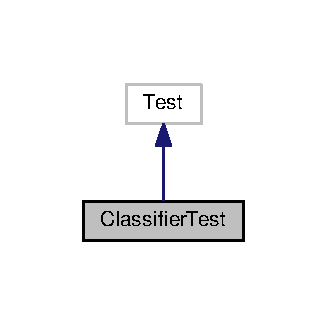
\includegraphics[width=157pt]{structClassifierTest__inherit__graph}
\end{center}
\end{figure}


Collaboration diagram for Classifier\+Test\+:
\nopagebreak
\begin{figure}[H]
\begin{center}
\leavevmode
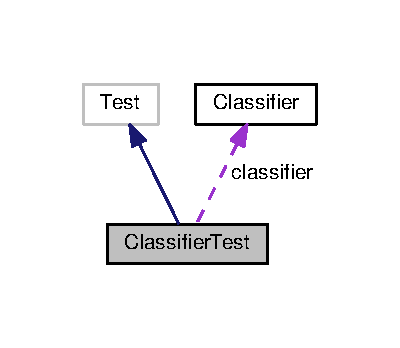
\includegraphics[width=192pt]{structClassifierTest__coll__graph}
\end{center}
\end{figure}
\subsection*{Public Member Functions}
\begin{DoxyCompactItemize}
\item 
\hyperlink{structClassifierTest_a44a8a84b2e0d51b914950a6333a13df7}{Classifier\+Test} ()
\item 
virtual \hyperlink{structClassifierTest_a12a8dd361b48330be8b4fedbd7570ea7}{$\sim$\+Classifier\+Test} ()
\end{DoxyCompactItemize}
\subsection*{Public Attributes}
\begin{DoxyCompactItemize}
\item 
\hyperlink{classClassifier}{Classifier} $\ast$ \hyperlink{structClassifierTest_a28f0a8fabef6be4190f293e2cf4644de}{classifier}
\end{DoxyCompactItemize}


\subsection{Constructor \& Destructor Documentation}
\index{Classifier\+Test@{Classifier\+Test}!Classifier\+Test@{Classifier\+Test}}
\index{Classifier\+Test@{Classifier\+Test}!Classifier\+Test@{Classifier\+Test}}
\subsubsection[{\texorpdfstring{Classifier\+Test()}{ClassifierTest()}}]{\setlength{\rightskip}{0pt plus 5cm}Classifier\+Test\+::\+Classifier\+Test (
\begin{DoxyParamCaption}
{}
\end{DoxyParamCaption}
)\hspace{0.3cm}{\ttfamily [inline]}}\hypertarget{structClassifierTest_a44a8a84b2e0d51b914950a6333a13df7}{}\label{structClassifierTest_a44a8a84b2e0d51b914950a6333a13df7}
\index{Classifier\+Test@{Classifier\+Test}!````~Classifier\+Test@{$\sim$\+Classifier\+Test}}
\index{````~Classifier\+Test@{$\sim$\+Classifier\+Test}!Classifier\+Test@{Classifier\+Test}}
\subsubsection[{\texorpdfstring{$\sim$\+Classifier\+Test()}{~ClassifierTest()}}]{\setlength{\rightskip}{0pt plus 5cm}virtual Classifier\+Test\+::$\sim$\+Classifier\+Test (
\begin{DoxyParamCaption}
{}
\end{DoxyParamCaption}
)\hspace{0.3cm}{\ttfamily [inline]}, {\ttfamily [virtual]}}\hypertarget{structClassifierTest_a12a8dd361b48330be8b4fedbd7570ea7}{}\label{structClassifierTest_a12a8dd361b48330be8b4fedbd7570ea7}


\subsection{Member Data Documentation}
\index{Classifier\+Test@{Classifier\+Test}!classifier@{classifier}}
\index{classifier@{classifier}!Classifier\+Test@{Classifier\+Test}}
\subsubsection[{\texorpdfstring{classifier}{classifier}}]{\setlength{\rightskip}{0pt plus 5cm}{\bf Classifier}$\ast$ Classifier\+Test\+::classifier}\hypertarget{structClassifierTest_a28f0a8fabef6be4190f293e2cf4644de}{}\label{structClassifierTest_a28f0a8fabef6be4190f293e2cf4644de}


The documentation for this struct was generated from the following file\+:\begin{DoxyCompactItemize}
\item 
test/\hyperlink{test_8cpp}{test.\+cpp}\end{DoxyCompactItemize}

\hypertarget{classContactInfo}{}\section{Contact\+Info Class Reference}
\label{classContactInfo}\index{Contact\+Info@{Contact\+Info}}


{\ttfamily \#include $<$Contact\+Info.\+hpp$>$}

\subsection*{Classes}
\begin{DoxyCompactItemize}
\item 
class \hyperlink{classContactInfo_1_1hpp}{hpp}
\begin{DoxyCompactList}\small\item\em This class stores the identity, name, and number of the contact. \end{DoxyCompactList}\end{DoxyCompactItemize}
\subsection*{Public Member Functions}
\begin{DoxyCompactItemize}
\item 
\hyperlink{classContactInfo_a4c76e92e4ef880a06af1404da32b3fa7}{Contact\+Info} ()
\item 
void \hyperlink{classContactInfo_a870acb96096d987a910fa3cc8022ac8f}{set\+Contact\+Info} (string Name, string Phone, string job)
\item 
std\+::string \hyperlink{classContactInfo_affb67018c3d052b91392eea9db29704c}{get\+Contact\+Info\+Phone} ()
\item 
std\+::string \hyperlink{classContactInfo_af07393e83fa33e470c40c419613bacf1}{get\+Contact\+Info\+Name} ()
\item 
std\+::string \hyperlink{classContactInfo_a8735facf207013b5f92f534cc6035242}{get\+Contact\+Info\+Job} ()
\end{DoxyCompactItemize}
\subsection*{Private Attributes}
\begin{DoxyCompactItemize}
\item 
std\+::string \hyperlink{classContactInfo_ae43d14159125871edf591d7a16a9aa15}{name}
\item 
std\+::string \hyperlink{classContactInfo_a74d162bbb4a96dff6794e644e6d62e38}{phone}
\item 
std\+::string \hyperlink{classContactInfo_a7126750ab0c8294f092278639d51c68a}{occupation}
\end{DoxyCompactItemize}


\subsection{Constructor \& Destructor Documentation}
\index{Contact\+Info@{Contact\+Info}!Contact\+Info@{Contact\+Info}}
\index{Contact\+Info@{Contact\+Info}!Contact\+Info@{Contact\+Info}}
\subsubsection[{\texorpdfstring{Contact\+Info()}{ContactInfo()}}]{\setlength{\rightskip}{0pt plus 5cm}Contact\+Info\+::\+Contact\+Info (
\begin{DoxyParamCaption}
{}
\end{DoxyParamCaption}
)\hspace{0.3cm}{\ttfamily [inline]}}\hypertarget{classContactInfo_a4c76e92e4ef880a06af1404da32b3fa7}{}\label{classContactInfo_a4c76e92e4ef880a06af1404da32b3fa7}


\subsection{Member Function Documentation}
\index{Contact\+Info@{Contact\+Info}!get\+Contact\+Info\+Job@{get\+Contact\+Info\+Job}}
\index{get\+Contact\+Info\+Job@{get\+Contact\+Info\+Job}!Contact\+Info@{Contact\+Info}}
\subsubsection[{\texorpdfstring{get\+Contact\+Info\+Job()}{getContactInfoJob()}}]{\setlength{\rightskip}{0pt plus 5cm}std\+::string Contact\+Info\+::get\+Contact\+Info\+Job (
\begin{DoxyParamCaption}
{}
\end{DoxyParamCaption}
)\hspace{0.3cm}{\ttfamily [inline]}}\hypertarget{classContactInfo_a8735facf207013b5f92f534cc6035242}{}\label{classContactInfo_a8735facf207013b5f92f534cc6035242}
\index{Contact\+Info@{Contact\+Info}!get\+Contact\+Info\+Name@{get\+Contact\+Info\+Name}}
\index{get\+Contact\+Info\+Name@{get\+Contact\+Info\+Name}!Contact\+Info@{Contact\+Info}}
\subsubsection[{\texorpdfstring{get\+Contact\+Info\+Name()}{getContactInfoName()}}]{\setlength{\rightskip}{0pt plus 5cm}std\+::string Contact\+Info\+::get\+Contact\+Info\+Name (
\begin{DoxyParamCaption}
{}
\end{DoxyParamCaption}
)\hspace{0.3cm}{\ttfamily [inline]}}\hypertarget{classContactInfo_af07393e83fa33e470c40c419613bacf1}{}\label{classContactInfo_af07393e83fa33e470c40c419613bacf1}
\index{Contact\+Info@{Contact\+Info}!get\+Contact\+Info\+Phone@{get\+Contact\+Info\+Phone}}
\index{get\+Contact\+Info\+Phone@{get\+Contact\+Info\+Phone}!Contact\+Info@{Contact\+Info}}
\subsubsection[{\texorpdfstring{get\+Contact\+Info\+Phone()}{getContactInfoPhone()}}]{\setlength{\rightskip}{0pt plus 5cm}std\+::string Contact\+Info\+::get\+Contact\+Info\+Phone (
\begin{DoxyParamCaption}
{}
\end{DoxyParamCaption}
)\hspace{0.3cm}{\ttfamily [inline]}}\hypertarget{classContactInfo_affb67018c3d052b91392eea9db29704c}{}\label{classContactInfo_affb67018c3d052b91392eea9db29704c}
\index{Contact\+Info@{Contact\+Info}!set\+Contact\+Info@{set\+Contact\+Info}}
\index{set\+Contact\+Info@{set\+Contact\+Info}!Contact\+Info@{Contact\+Info}}
\subsubsection[{\texorpdfstring{set\+Contact\+Info(string Name, string Phone, string job)}{setContactInfo(string Name, string Phone, string job)}}]{\setlength{\rightskip}{0pt plus 5cm}void Contact\+Info\+::set\+Contact\+Info (
\begin{DoxyParamCaption}
\item[{string}]{Name, }
\item[{string}]{Phone, }
\item[{string}]{job}
\end{DoxyParamCaption}
)\hspace{0.3cm}{\ttfamily [inline]}}\hypertarget{classContactInfo_a870acb96096d987a910fa3cc8022ac8f}{}\label{classContactInfo_a870acb96096d987a910fa3cc8022ac8f}


\subsection{Member Data Documentation}
\index{Contact\+Info@{Contact\+Info}!name@{name}}
\index{name@{name}!Contact\+Info@{Contact\+Info}}
\subsubsection[{\texorpdfstring{name}{name}}]{\setlength{\rightskip}{0pt plus 5cm}std\+::string Contact\+Info\+::name\hspace{0.3cm}{\ttfamily [private]}}\hypertarget{classContactInfo_ae43d14159125871edf591d7a16a9aa15}{}\label{classContactInfo_ae43d14159125871edf591d7a16a9aa15}
\index{Contact\+Info@{Contact\+Info}!occupation@{occupation}}
\index{occupation@{occupation}!Contact\+Info@{Contact\+Info}}
\subsubsection[{\texorpdfstring{occupation}{occupation}}]{\setlength{\rightskip}{0pt plus 5cm}std\+::string Contact\+Info\+::occupation\hspace{0.3cm}{\ttfamily [private]}}\hypertarget{classContactInfo_a7126750ab0c8294f092278639d51c68a}{}\label{classContactInfo_a7126750ab0c8294f092278639d51c68a}
\index{Contact\+Info@{Contact\+Info}!phone@{phone}}
\index{phone@{phone}!Contact\+Info@{Contact\+Info}}
\subsubsection[{\texorpdfstring{phone}{phone}}]{\setlength{\rightskip}{0pt plus 5cm}std\+::string Contact\+Info\+::phone\hspace{0.3cm}{\ttfamily [private]}}\hypertarget{classContactInfo_a74d162bbb4a96dff6794e644e6d62e38}{}\label{classContactInfo_a74d162bbb4a96dff6794e644e6d62e38}


The documentation for this class was generated from the following file\+:\begin{DoxyCompactItemize}
\item 
include/\hyperlink{ContactInfo_8hpp}{Contact\+Info.\+hpp}\end{DoxyCompactItemize}

\hypertarget{classDetectedImg}{}\section{Detected\+Img Class Reference}
\label{classDetectedImg}\index{Detected\+Img@{Detected\+Img}}


{\ttfamily \#include $<$Detected\+Img.\+hpp$>$}

\subsection*{Public Member Functions}
\begin{DoxyCompactItemize}
\item 
\hyperlink{classDetectedImg_aacfdecaa861ddc2ce7747d1f6e2f2345}{Detected\+Img} ()
\item 
void \hyperlink{classDetectedImg_a625f4bb19646eb053e866391bea3d1d7}{load\+Imgs} (cv\+::\+Mat \&)
\item 
cv\+::\+Mat \& \hyperlink{classDetectedImg_ab9978594a666a1886902c26b80536987}{get\+Imgs} (int ord)
\item 
int \hyperlink{classDetectedImg_a7814c694d6b56bcf521e07fcb5b8ab60}{view\+Result} (int order)
\item 
void \hyperlink{classDetectedImg_afd084418ea8fed43f56c6596f80899d1}{set\+Result} (int)
\item 
int \hyperlink{classDetectedImg_a14ad13a688df84c69e11265af48f517c}{get\+Size} ()
\end{DoxyCompactItemize}
\subsection*{Private Attributes}
\begin{DoxyCompactItemize}
\item 
std\+::vector$<$ cv\+::\+Mat $>$ \hyperlink{classDetectedImg_a5954f5c930b5c041debd10338d02f195}{detected\+Imgs}
\item 
std\+::vector$<$ int $>$ \hyperlink{classDetectedImg_a498ad454ddc09681abfef4b6ac1da3a1}{result}
\end{DoxyCompactItemize}


\subsection{Constructor \& Destructor Documentation}
\index{Detected\+Img@{Detected\+Img}!Detected\+Img@{Detected\+Img}}
\index{Detected\+Img@{Detected\+Img}!Detected\+Img@{Detected\+Img}}
\subsubsection[{\texorpdfstring{Detected\+Img()}{DetectedImg()}}]{\setlength{\rightskip}{0pt plus 5cm}Detected\+Img\+::\+Detected\+Img (
\begin{DoxyParamCaption}
{}
\end{DoxyParamCaption}
)}\hypertarget{classDetectedImg_aacfdecaa861ddc2ce7747d1f6e2f2345}{}\label{classDetectedImg_aacfdecaa861ddc2ce7747d1f6e2f2345}


\subsection{Member Function Documentation}
\index{Detected\+Img@{Detected\+Img}!get\+Imgs@{get\+Imgs}}
\index{get\+Imgs@{get\+Imgs}!Detected\+Img@{Detected\+Img}}
\subsubsection[{\texorpdfstring{get\+Imgs(int ord)}{getImgs(int ord)}}]{\setlength{\rightskip}{0pt plus 5cm}cv\+::\+Mat \& Detected\+Img\+::get\+Imgs (
\begin{DoxyParamCaption}
\item[{int}]{ord}
\end{DoxyParamCaption}
)}\hypertarget{classDetectedImg_ab9978594a666a1886902c26b80536987}{}\label{classDetectedImg_ab9978594a666a1886902c26b80536987}
Retract images from detected image vector 
\begin{DoxyParams}{Parameters}
{\em cv\+::\+Mat} & \\
\hline
\end{DoxyParams}
\begin{DoxyReturn}{Returns}
cv\+::\+Mat at specific index in the vector
\end{DoxyReturn}
\index{Detected\+Img@{Detected\+Img}!get\+Size@{get\+Size}}
\index{get\+Size@{get\+Size}!Detected\+Img@{Detected\+Img}}
\subsubsection[{\texorpdfstring{get\+Size()}{getSize()}}]{\setlength{\rightskip}{0pt plus 5cm}int Detected\+Img\+::get\+Size (
\begin{DoxyParamCaption}
{}
\end{DoxyParamCaption}
)\hspace{0.3cm}{\ttfamily [inline]}}\hypertarget{classDetectedImg_a14ad13a688df84c69e11265af48f517c}{}\label{classDetectedImg_a14ad13a688df84c69e11265af48f517c}
\index{Detected\+Img@{Detected\+Img}!load\+Imgs@{load\+Imgs}}
\index{load\+Imgs@{load\+Imgs}!Detected\+Img@{Detected\+Img}}
\subsubsection[{\texorpdfstring{load\+Imgs(cv\+::\+Mat \&)}{loadImgs(cv::Mat &)}}]{\setlength{\rightskip}{0pt plus 5cm}void Detected\+Img\+::load\+Imgs (
\begin{DoxyParamCaption}
\item[{cv\+::\+Mat \&}]{img}
\end{DoxyParamCaption}
)}\hypertarget{classDetectedImg_a625f4bb19646eb053e866391bea3d1d7}{}\label{classDetectedImg_a625f4bb19646eb053e866391bea3d1d7}
Store images from detected image vector 
\begin{DoxyParams}{Parameters}
{\em cv\+::\+Mat} & \\
\hline
\end{DoxyParams}
\begin{DoxyReturn}{Returns}
none
\end{DoxyReturn}
\index{Detected\+Img@{Detected\+Img}!set\+Result@{set\+Result}}
\index{set\+Result@{set\+Result}!Detected\+Img@{Detected\+Img}}
\subsubsection[{\texorpdfstring{set\+Result(int)}{setResult(int)}}]{\setlength{\rightskip}{0pt plus 5cm}void Detected\+Img\+::set\+Result (
\begin{DoxyParamCaption}
\item[{int}]{rest}
\end{DoxyParamCaption}
)}\hypertarget{classDetectedImg_afd084418ea8fed43f56c6596f80899d1}{}\label{classDetectedImg_afd084418ea8fed43f56c6596f80899d1}
Set S\+VM result for each image 
\begin{DoxyParams}{Parameters}
{\em S\+VM} & result integer \\
\hline
\end{DoxyParams}
\begin{DoxyReturn}{Returns}
none
\end{DoxyReturn}
\index{Detected\+Img@{Detected\+Img}!view\+Result@{view\+Result}}
\index{view\+Result@{view\+Result}!Detected\+Img@{Detected\+Img}}
\subsubsection[{\texorpdfstring{view\+Result(int order)}{viewResult(int order)}}]{\setlength{\rightskip}{0pt plus 5cm}int Detected\+Img\+::view\+Result (
\begin{DoxyParamCaption}
\item[{int}]{order}
\end{DoxyParamCaption}
)}\hypertarget{classDetectedImg_a7814c694d6b56bcf521e07fcb5b8ab60}{}\label{classDetectedImg_a7814c694d6b56bcf521e07fcb5b8ab60}
Get S\+VM result for each image 
\begin{DoxyParams}{Parameters}
{\em S\+VM} & result integer \\
\hline
\end{DoxyParams}
\begin{DoxyReturn}{Returns}
S\+VM result integer at specified index in the vector
\end{DoxyReturn}


\subsection{Member Data Documentation}
\index{Detected\+Img@{Detected\+Img}!detected\+Imgs@{detected\+Imgs}}
\index{detected\+Imgs@{detected\+Imgs}!Detected\+Img@{Detected\+Img}}
\subsubsection[{\texorpdfstring{detected\+Imgs}{detectedImgs}}]{\setlength{\rightskip}{0pt plus 5cm}std\+::vector$<$cv\+::\+Mat$>$ Detected\+Img\+::detected\+Imgs\hspace{0.3cm}{\ttfamily [private]}}\hypertarget{classDetectedImg_a5954f5c930b5c041debd10338d02f195}{}\label{classDetectedImg_a5954f5c930b5c041debd10338d02f195}
\index{Detected\+Img@{Detected\+Img}!result@{result}}
\index{result@{result}!Detected\+Img@{Detected\+Img}}
\subsubsection[{\texorpdfstring{result}{result}}]{\setlength{\rightskip}{0pt plus 5cm}std\+::vector$<$int$>$ Detected\+Img\+::result\hspace{0.3cm}{\ttfamily [private]}}\hypertarget{classDetectedImg_a498ad454ddc09681abfef4b6ac1da3a1}{}\label{classDetectedImg_a498ad454ddc09681abfef4b6ac1da3a1}


The documentation for this class was generated from the following files\+:\begin{DoxyCompactItemize}
\item 
include/\hyperlink{DetectedImg_8hpp}{Detected\+Img.\+hpp}\item 
app/\hyperlink{DetectedImg_8cpp}{Detected\+Img.\+cpp}\end{DoxyCompactItemize}

\hypertarget{structDetectedTest}{}\section{Detected\+Test Struct Reference}
\label{structDetectedTest}\index{Detected\+Test@{Detected\+Test}}


Inheritance diagram for Detected\+Test\+:
\nopagebreak
\begin{figure}[H]
\begin{center}
\leavevmode
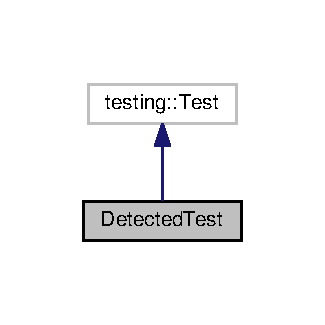
\includegraphics[width=156pt]{structDetectedTest__inherit__graph}
\end{center}
\end{figure}


Collaboration diagram for Detected\+Test\+:
\nopagebreak
\begin{figure}[H]
\begin{center}
\leavevmode
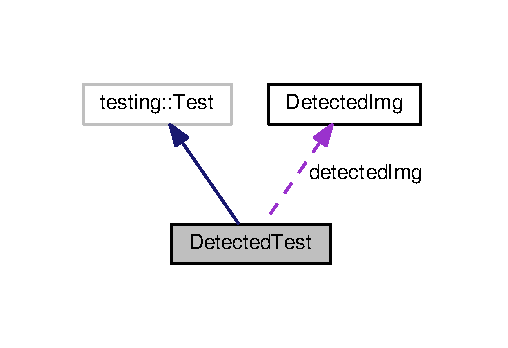
\includegraphics[width=244pt]{structDetectedTest__coll__graph}
\end{center}
\end{figure}
\subsection*{Public Member Functions}
\begin{DoxyCompactItemize}
\item 
\hyperlink{structDetectedTest_a748e3dfbb0203c2f4e7b7970fbbcd39c}{Detected\+Test} ()
\item 
virtual \hyperlink{structDetectedTest_aae6a3bf0303439e9d4d7d390770a6fd1}{$\sim$\+Detected\+Test} ()
\end{DoxyCompactItemize}
\subsection*{Public Attributes}
\begin{DoxyCompactItemize}
\item 
\hyperlink{classDetectedImg}{Detected\+Img} $\ast$ \hyperlink{structDetectedTest_a626f16728a762f1d3592cb063130a28a}{detected\+Img}
\end{DoxyCompactItemize}


\subsection{Constructor \& Destructor Documentation}
\index{Detected\+Test@{Detected\+Test}!Detected\+Test@{Detected\+Test}}
\index{Detected\+Test@{Detected\+Test}!Detected\+Test@{Detected\+Test}}
\subsubsection[{\texorpdfstring{Detected\+Test()}{DetectedTest()}}]{\setlength{\rightskip}{0pt plus 5cm}Detected\+Test\+::\+Detected\+Test (
\begin{DoxyParamCaption}
{}
\end{DoxyParamCaption}
)\hspace{0.3cm}{\ttfamily [inline]}}\hypertarget{structDetectedTest_a748e3dfbb0203c2f4e7b7970fbbcd39c}{}\label{structDetectedTest_a748e3dfbb0203c2f4e7b7970fbbcd39c}
\index{Detected\+Test@{Detected\+Test}!````~Detected\+Test@{$\sim$\+Detected\+Test}}
\index{````~Detected\+Test@{$\sim$\+Detected\+Test}!Detected\+Test@{Detected\+Test}}
\subsubsection[{\texorpdfstring{$\sim$\+Detected\+Test()}{~DetectedTest()}}]{\setlength{\rightskip}{0pt plus 5cm}virtual Detected\+Test\+::$\sim$\+Detected\+Test (
\begin{DoxyParamCaption}
{}
\end{DoxyParamCaption}
)\hspace{0.3cm}{\ttfamily [inline]}, {\ttfamily [virtual]}}\hypertarget{structDetectedTest_aae6a3bf0303439e9d4d7d390770a6fd1}{}\label{structDetectedTest_aae6a3bf0303439e9d4d7d390770a6fd1}


\subsection{Member Data Documentation}
\index{Detected\+Test@{Detected\+Test}!detected\+Img@{detected\+Img}}
\index{detected\+Img@{detected\+Img}!Detected\+Test@{Detected\+Test}}
\subsubsection[{\texorpdfstring{detected\+Img}{detectedImg}}]{\setlength{\rightskip}{0pt plus 5cm}{\bf Detected\+Img}$\ast$ Detected\+Test\+::detected\+Img}\hypertarget{structDetectedTest_a626f16728a762f1d3592cb063130a28a}{}\label{structDetectedTest_a626f16728a762f1d3592cb063130a28a}


The documentation for this struct was generated from the following file\+:\begin{DoxyCompactItemize}
\item 
test/\hyperlink{test_8cpp}{test.\+cpp}\end{DoxyCompactItemize}

\hypertarget{classClassifer_1_1h}{}\section{Classifer\+:\+:h Class Reference}
\label{classClassifer_1_1h}\index{Classifer\+::h@{Classifer\+::h}}


\hyperlink{classClassifier}{Classifier} class generates binary class classifier from image samples  to train linear S\+VM.  




{\ttfamily \#include $<$Classifier.\+hpp$>$}



\subsection{Detailed Description}
\hyperlink{classClassifier}{Classifier} class generates binary class classifier from image samples  to train linear S\+VM. 

\begin{DoxyCopyright}{Copyright}
Copyright 2017 Yuyu Hsueh. All rights reserved.
\end{DoxyCopyright}
A binary classifier class is created to train to detect dogs/blind humans in a random images. 

The documentation for this class was generated from the following file\+:\begin{DoxyCompactItemize}
\item 
include/\hyperlink{Classifier_8hpp}{Classifier.\+hpp}\end{DoxyCompactItemize}

\hypertarget{classContactInfo_1_1hpp}{}\section{Contact\+Info\+:\+:hpp Class Reference}
\label{classContactInfo_1_1hpp}\index{Contact\+Info\+::hpp@{Contact\+Info\+::hpp}}


This class stores the identity, name, and number of the contact.  




{\ttfamily \#include $<$Contact\+Info.\+hpp$>$}



\subsection{Detailed Description}
This class stores the identity, name, and number of the contact. 

\begin{DoxyCopyright}{Copyright}
Copyright 2017 Yuyu Hsueh. All rights reserved. 
\end{DoxyCopyright}


The documentation for this class was generated from the following file\+:\begin{DoxyCompactItemize}
\item 
include/\hyperlink{ContactInfo_8hpp}{Contact\+Info.\+hpp}\end{DoxyCompactItemize}

\chapter{File Documentation}
\hypertarget{Classifier_8cpp}{}\section{app/\+Classifier.cpp File Reference}
\label{Classifier_8cpp}\index{app/\+Classifier.\+cpp@{app/\+Classifier.\+cpp}}


This is cpp file for \hyperlink{classClassifier}{Classifier} class which extracts H\+OG features from sample images and trains binary class classifier for dogs and supposedly humans.  


{\ttfamily \#include \char`\"{}Classifier.\+hpp\char`\"{}}\\*
{\ttfamily \#include $<$boost/filesystem.\+hpp$>$}\\*
{\ttfamily \#include $<$opencv2/core/core.\+hpp$>$}\\*
{\ttfamily \#include $<$opencv2/opencv.\+hpp$>$}\\*
{\ttfamily \#include $<$opencv2/objdetect/objdetect.\+hpp$>$}\\*
{\ttfamily \#include $<$iostream$>$}\\*
{\ttfamily \#include $<$string$>$}\\*
{\ttfamily \#include $<$vector$>$}\\*
Include dependency graph for Classifier.\+cpp\+:
\nopagebreak
\begin{figure}[H]
\begin{center}
\leavevmode
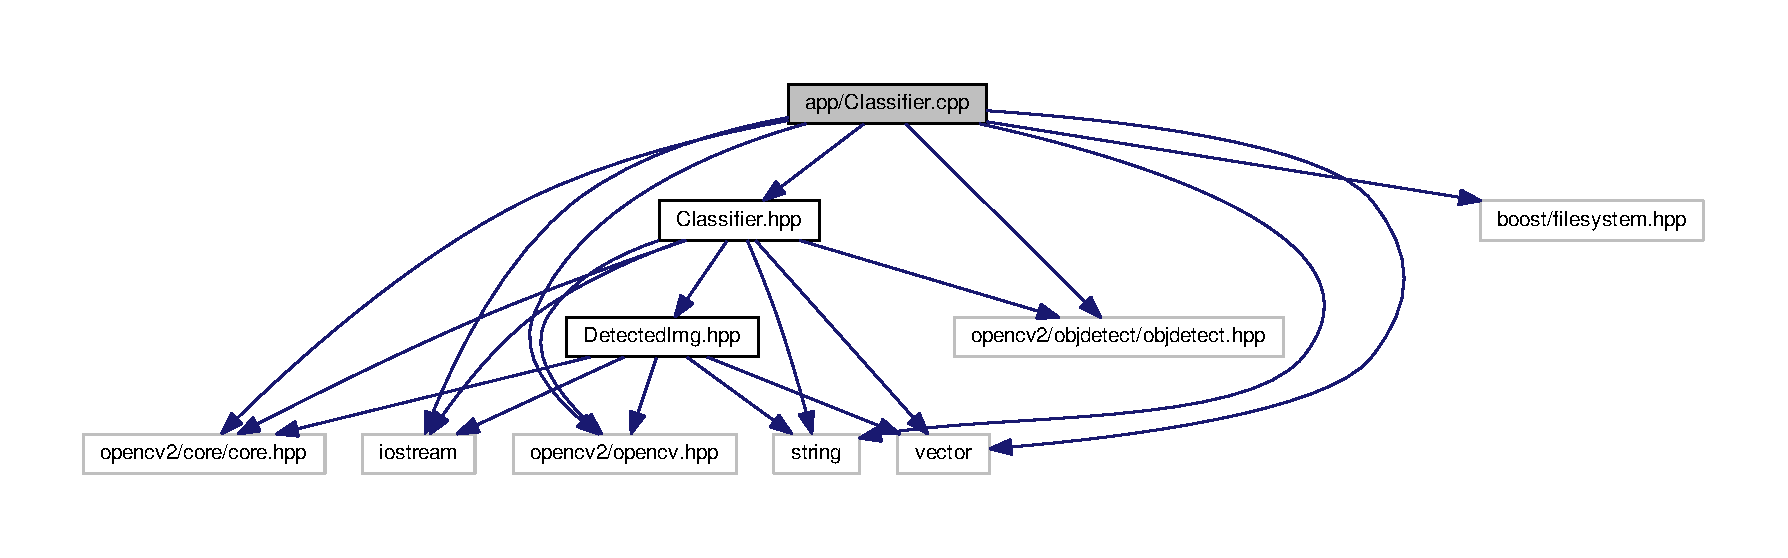
\includegraphics[width=350pt]{Classifier_8cpp__incl}
\end{center}
\end{figure}


\subsection{Detailed Description}
This is cpp file for \hyperlink{classClassifier}{Classifier} class which extracts H\+OG features from sample images and trains binary class classifier for dogs and supposedly humans. 

\hyperlink{classClassifier}{Classifier} class that uses the extracted H\+OG features of the sample images to train linear S\+VM.

\begin{DoxyAuthor}{Author}
Yuyu Hsueh 
\end{DoxyAuthor}
\begin{DoxyCopyright}{Copyright}
Copyright 2017 Yuyu Hsueh. All rights reserved. Licensor hereby grants Licensee a Sublicensable, Non-\/assignable \& non-\/transferable, Pepetual, Commercial, Royalty free. Including the rights to create but not distribute derivative works, Non-\/exclusive license, all with accordance with the terms set forth and other legal restrictions set forth in 3rd party software used while running Software.

Copyright 2017 Yuyu Hsueh. All rights reserved.
\end{DoxyCopyright}
A binary classifier class is created to train to detect dogs in a random images. 
\hypertarget{demo_8cpp}{}\section{app/demo.cpp File Reference}
\label{demo_8cpp}\index{app/demo.\+cpp@{app/demo.\+cpp}}


This is where classifier class is called and set up.  


{\ttfamily \#include $<$string$>$}\\*
{\ttfamily \#include $<$vector$>$}\\*
{\ttfamily \#include $<$memory$>$}\\*
{\ttfamily \#include \char`\"{}Classifier.\+hpp\char`\"{}}\\*
Include dependency graph for demo.\+cpp\+:
\nopagebreak
\begin{figure}[H]
\begin{center}
\leavevmode
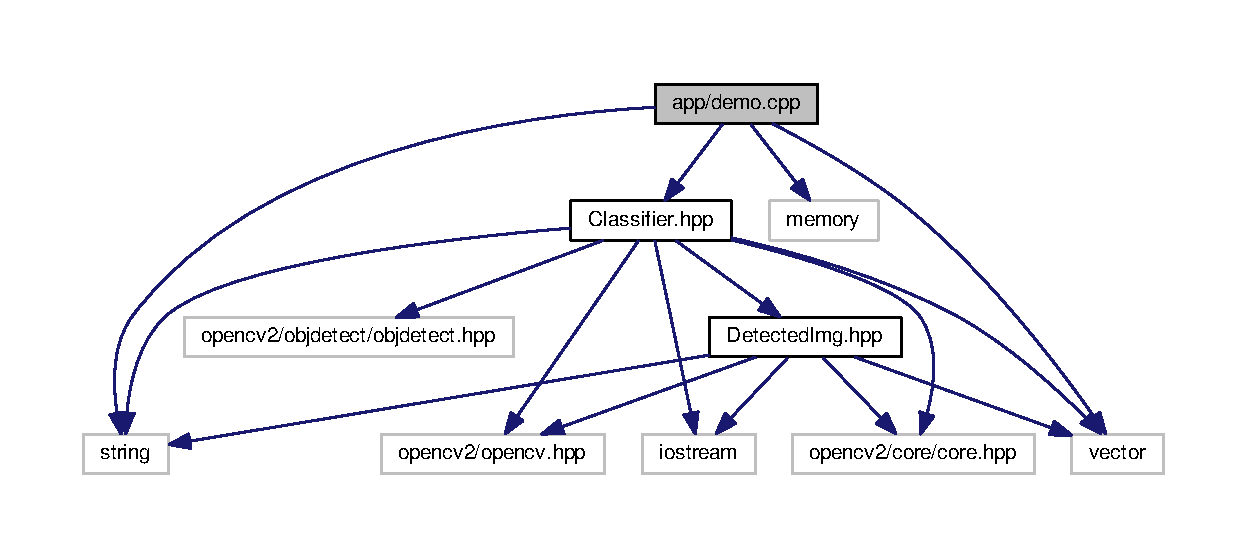
\includegraphics[width=350pt]{demo_8cpp__incl}
\end{center}
\end{figure}
\subsection*{Functions}
\begin{DoxyCompactItemize}
\item 
void \hyperlink{demo_8cpp_a1aadb6a82ef4e96267850eb89f947819}{dog\+Classifier\+Init} (\hyperlink{classDetectedImg}{Detected\+Img} \&imgs, int mode)
\item 
int \hyperlink{demo_8cpp_ae66f6b31b5ad750f1fe042a706a4e3d4}{main} ()
\end{DoxyCompactItemize}


\subsection{Detailed Description}
This is where classifier class is called and set up. 

\begin{DoxyAuthor}{Author}
Yuyu Hsueh 
\end{DoxyAuthor}
\begin{DoxyCopyright}{Copyright}
Copyright 2017 Yuyu Hsueh. All rights reserved. Licensor hereby grants Licensee a Sublicensable, Non-\/assignable \& non-\/transferable, Pepetual, Commercial, Royalty free. Including the rights to create but not distribute derivative works, Non-\/exclusive license, all with accordance with the terms set forth and other legal restrictions set forth in 3rd party software used while running Software. 
\end{DoxyCopyright}


\subsection{Function Documentation}
\index{demo.\+cpp@{demo.\+cpp}!dog\+Classifier\+Init@{dog\+Classifier\+Init}}
\index{dog\+Classifier\+Init@{dog\+Classifier\+Init}!demo.\+cpp@{demo.\+cpp}}
\subsubsection[{\texorpdfstring{dog\+Classifier\+Init(\+Detected\+Img \&imgs, int mode)}{dogClassifierInit(DetectedImg &imgs, int mode)}}]{\setlength{\rightskip}{0pt plus 5cm}void dog\+Classifier\+Init (
\begin{DoxyParamCaption}
\item[{{\bf Detected\+Img} \&}]{imgs, }
\item[{int}]{mode}
\end{DoxyParamCaption}
)}\hypertarget{demo_8cpp_a1aadb6a82ef4e96267850eb89f947819}{}\label{demo_8cpp_a1aadb6a82ef4e96267850eb89f947819}
Dog classifier initialization. Mode 1 loads classifier. Mode 2 trains new classifier. 
\begin{DoxyParams}{Parameters}
{\em \hyperlink{classDetectedImg}{Detected\+Img},int} & \\
\hline
\end{DoxyParams}
\begin{DoxyReturn}{Returns}
none
\end{DoxyReturn}
\index{demo.\+cpp@{demo.\+cpp}!main@{main}}
\index{main@{main}!demo.\+cpp@{demo.\+cpp}}
\subsubsection[{\texorpdfstring{main()}{main()}}]{\setlength{\rightskip}{0pt plus 5cm}int main (
\begin{DoxyParamCaption}
{}
\end{DoxyParamCaption}
)}\hypertarget{demo_8cpp_ae66f6b31b5ad750f1fe042a706a4e3d4}{}\label{demo_8cpp_ae66f6b31b5ad750f1fe042a706a4e3d4}
In this demo, three street views are tested, and the results from S\+VM analysis will be returned along with the image. 
\begin{DoxyParams}{Parameters}
{\em none} & \\
\hline
\end{DoxyParams}
\begin{DoxyReturn}{Returns}
none
\end{DoxyReturn}
$<$ mode 0\+: train classifier; mode 1\+: load pretrained classifier 
\hypertarget{DetectedImg_8cpp}{}\section{app/\+Detected\+Img.cpp File Reference}
\label{DetectedImg_8cpp}\index{app/\+Detected\+Img.\+cpp@{app/\+Detected\+Img.\+cpp}}


This is cpp file for \hyperlink{classDetectedImg}{Detected\+Img} class which stores the images and its results after the S\+VM analysis.  


{\ttfamily \#include $<$opencv2/core/core.\+hpp$>$}\\*
{\ttfamily \#include $<$opencv2/opencv.\+hpp$>$}\\*
{\ttfamily \#include $<$iostream$>$}\\*
{\ttfamily \#include $<$string$>$}\\*
{\ttfamily \#include $<$vector$>$}\\*
{\ttfamily \#include \char`\"{}Detected\+Img.\+hpp\char`\"{}}\\*
Include dependency graph for Detected\+Img.\+cpp\+:
\nopagebreak
\begin{figure}[H]
\begin{center}
\leavevmode
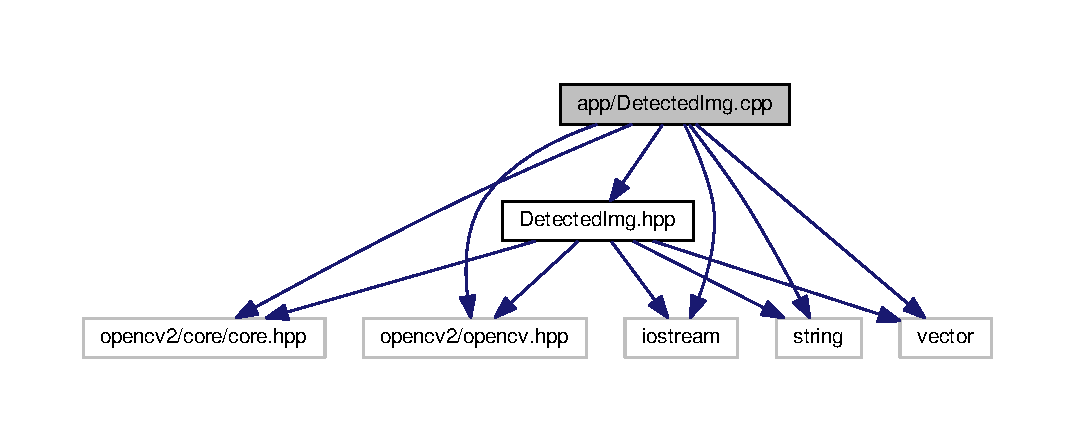
\includegraphics[width=350pt]{DetectedImg_8cpp__incl}
\end{center}
\end{figure}


\subsection{Detailed Description}
This is cpp file for \hyperlink{classDetectedImg}{Detected\+Img} class which stores the images and its results after the S\+VM analysis. 

\begin{DoxyAuthor}{Author}
Yuyu Hsueh 
\end{DoxyAuthor}
\begin{DoxyCopyright}{Copyright}
Copyright 2017 Yuyu Hsueh. All rights reserved. Licensor hereby grants Licensee a Sublicensable, Non-\/assignable \& non-\/transferable, Pepetual, Commercial, Royalty free. Including the rights to create but not distribute derivative works, Non-\/exclusive license, all with accordance with the terms set forth and other legal restrictions set forth in 3rd party software used while running Software. 
\end{DoxyCopyright}

\hypertarget{CMakeCXXCompilerId_8cpp}{}\section{build/\+C\+Make\+Files/3.5.1/\+Compiler\+Id\+C\+X\+X/\+C\+Make\+C\+X\+X\+Compiler\+Id.cpp File Reference}
\label{CMakeCXXCompilerId_8cpp}\index{build/\+C\+Make\+Files/3.\+5.\+1/\+Compiler\+Id\+C\+X\+X/\+C\+Make\+C\+X\+X\+Compiler\+Id.\+cpp@{build/\+C\+Make\+Files/3.\+5.\+1/\+Compiler\+Id\+C\+X\+X/\+C\+Make\+C\+X\+X\+Compiler\+Id.\+cpp}}
\subsection*{Macros}
\begin{DoxyCompactItemize}
\item 
\#define \hyperlink{CMakeCXXCompilerId_8cpp_a81dee0709ded976b2e0319239f72d174}{C\+O\+M\+P\+I\+L\+E\+R\+\_\+\+ID}~\char`\"{}\char`\"{}
\item 
\#define \hyperlink{CMakeCXXCompilerId_8cpp_a2ae9b72bb13abaabfcf2ee0ba7d3fa1d}{S\+T\+R\+I\+N\+G\+I\+F\+Y\+\_\+\+H\+E\+L\+P\+ER}(X)~\#X
\item 
\#define \hyperlink{CMakeCXXCompilerId_8cpp_a43e1cad902b6477bec893cb6430bd6c8}{S\+T\+R\+I\+N\+G\+I\+FY}(X)~\hyperlink{CMakeCXXCompilerId_8cpp_a2ae9b72bb13abaabfcf2ee0ba7d3fa1d}{S\+T\+R\+I\+N\+G\+I\+F\+Y\+\_\+\+H\+E\+L\+P\+ER}(X)
\item 
\#define \hyperlink{CMakeCXXCompilerId_8cpp_adbc5372f40838899018fadbc89bd588b}{P\+L\+A\+T\+F\+O\+R\+M\+\_\+\+ID}~\char`\"{}\char`\"{}
\item 
\#define \hyperlink{CMakeCXXCompilerId_8cpp_aba35d0d200deaeb06aee95ca297acb28}{A\+R\+C\+H\+I\+T\+E\+C\+T\+U\+R\+E\+\_\+\+ID}~\char`\"{}\char`\"{}
\item 
\#define \hyperlink{CMakeCXXCompilerId_8cpp_ad1280362da42492bbc11aa78cbf776ad}{D\+EC}(n)
\item 
\#define \hyperlink{CMakeCXXCompilerId_8cpp_a46d5d95daa1bef867bd0179594310ed5}{H\+EX}(n)
\end{DoxyCompactItemize}
\subsection*{Functions}
\begin{DoxyCompactItemize}
\item 
int \hyperlink{CMakeCXXCompilerId_8cpp_a0ddf1224851353fc92bfbff6f499fa97}{main} (int argc, char $\ast$argv\mbox{[}$\,$\mbox{]})
\end{DoxyCompactItemize}
\subsection*{Variables}
\begin{DoxyCompactItemize}
\item 
char const $\ast$ \hyperlink{CMakeCXXCompilerId_8cpp_a4b0efeb7a5d59313986b3a0390f050f6}{info\+\_\+compiler} = \char`\"{}I\+N\+FO\char`\"{} \char`\"{}\+:\char`\"{} \char`\"{}compiler\mbox{[}\char`\"{} C\+O\+M\+P\+I\+L\+E\+R\+\_\+\+ID \char`\"{}\mbox{]}\char`\"{}
\item 
char const $\ast$ \hyperlink{CMakeCXXCompilerId_8cpp_a2321403dee54ee23f0c2fa849c60f7d4}{info\+\_\+platform} = \char`\"{}I\+N\+FO\char`\"{} \char`\"{}\+:\char`\"{} \char`\"{}platform\mbox{[}\char`\"{} P\+L\+A\+T\+F\+O\+R\+M\+\_\+\+ID \char`\"{}\mbox{]}\char`\"{}
\item 
char const $\ast$ \hyperlink{CMakeCXXCompilerId_8cpp_a59647e99d304ed33b15cb284c27ed391}{info\+\_\+arch} = \char`\"{}I\+N\+FO\char`\"{} \char`\"{}\+:\char`\"{} \char`\"{}arch\mbox{[}\char`\"{} A\+R\+C\+H\+I\+T\+E\+C\+T\+U\+R\+E\+\_\+\+ID \char`\"{}\mbox{]}\char`\"{}
\item 
const char $\ast$ \hyperlink{CMakeCXXCompilerId_8cpp_a1ce162bad2fe6966ac8b33cc19e120b8}{info\+\_\+language\+\_\+dialect\+\_\+default}
\end{DoxyCompactItemize}


\subsection{Macro Definition Documentation}
\index{C\+Make\+C\+X\+X\+Compiler\+Id.\+cpp@{C\+Make\+C\+X\+X\+Compiler\+Id.\+cpp}!A\+R\+C\+H\+I\+T\+E\+C\+T\+U\+R\+E\+\_\+\+ID@{A\+R\+C\+H\+I\+T\+E\+C\+T\+U\+R\+E\+\_\+\+ID}}
\index{A\+R\+C\+H\+I\+T\+E\+C\+T\+U\+R\+E\+\_\+\+ID@{A\+R\+C\+H\+I\+T\+E\+C\+T\+U\+R\+E\+\_\+\+ID}!C\+Make\+C\+X\+X\+Compiler\+Id.\+cpp@{C\+Make\+C\+X\+X\+Compiler\+Id.\+cpp}}
\subsubsection[{\texorpdfstring{A\+R\+C\+H\+I\+T\+E\+C\+T\+U\+R\+E\+\_\+\+ID}{ARCHITECTURE_ID}}]{\setlength{\rightskip}{0pt plus 5cm}\#define A\+R\+C\+H\+I\+T\+E\+C\+T\+U\+R\+E\+\_\+\+ID~\char`\"{}\char`\"{}}\hypertarget{CMakeCXXCompilerId_8cpp_aba35d0d200deaeb06aee95ca297acb28}{}\label{CMakeCXXCompilerId_8cpp_aba35d0d200deaeb06aee95ca297acb28}
\index{C\+Make\+C\+X\+X\+Compiler\+Id.\+cpp@{C\+Make\+C\+X\+X\+Compiler\+Id.\+cpp}!C\+O\+M\+P\+I\+L\+E\+R\+\_\+\+ID@{C\+O\+M\+P\+I\+L\+E\+R\+\_\+\+ID}}
\index{C\+O\+M\+P\+I\+L\+E\+R\+\_\+\+ID@{C\+O\+M\+P\+I\+L\+E\+R\+\_\+\+ID}!C\+Make\+C\+X\+X\+Compiler\+Id.\+cpp@{C\+Make\+C\+X\+X\+Compiler\+Id.\+cpp}}
\subsubsection[{\texorpdfstring{C\+O\+M\+P\+I\+L\+E\+R\+\_\+\+ID}{COMPILER_ID}}]{\setlength{\rightskip}{0pt plus 5cm}\#define C\+O\+M\+P\+I\+L\+E\+R\+\_\+\+ID~\char`\"{}\char`\"{}}\hypertarget{CMakeCXXCompilerId_8cpp_a81dee0709ded976b2e0319239f72d174}{}\label{CMakeCXXCompilerId_8cpp_a81dee0709ded976b2e0319239f72d174}
\index{C\+Make\+C\+X\+X\+Compiler\+Id.\+cpp@{C\+Make\+C\+X\+X\+Compiler\+Id.\+cpp}!D\+EC@{D\+EC}}
\index{D\+EC@{D\+EC}!C\+Make\+C\+X\+X\+Compiler\+Id.\+cpp@{C\+Make\+C\+X\+X\+Compiler\+Id.\+cpp}}
\subsubsection[{\texorpdfstring{D\+EC}{DEC}}]{\setlength{\rightskip}{0pt plus 5cm}\#define D\+EC(
\begin{DoxyParamCaption}
\item[{}]{n}
\end{DoxyParamCaption}
)}\hypertarget{CMakeCXXCompilerId_8cpp_ad1280362da42492bbc11aa78cbf776ad}{}\label{CMakeCXXCompilerId_8cpp_ad1280362da42492bbc11aa78cbf776ad}
{\bfseries Value\+:}
\begin{DoxyCode}
(\textcolor{charliteral}{'0'} + (((n) / 10000000)%10)), \(\backslash\)
  (\textcolor{charliteral}{'0'} + (((n) / 1000000)%10)),  \(\backslash\)
  (\textcolor{charliteral}{'0'} + (((n) / 100000)%10)),   \(\backslash\)
  (\textcolor{charliteral}{'0'} + (((n) / 10000)%10)),    \(\backslash\)
  (\textcolor{charliteral}{'0'} + (((n) / 1000)%10)),     \(\backslash\)
  (\textcolor{charliteral}{'0'} + (((n) / 100)%10)),      \(\backslash\)
  (\textcolor{charliteral}{'0'} + (((n) / 10)%10)),       \(\backslash\)
  (\textcolor{charliteral}{'0'} +  ((n) % 10))
\end{DoxyCode}
\index{C\+Make\+C\+X\+X\+Compiler\+Id.\+cpp@{C\+Make\+C\+X\+X\+Compiler\+Id.\+cpp}!H\+EX@{H\+EX}}
\index{H\+EX@{H\+EX}!C\+Make\+C\+X\+X\+Compiler\+Id.\+cpp@{C\+Make\+C\+X\+X\+Compiler\+Id.\+cpp}}
\subsubsection[{\texorpdfstring{H\+EX}{HEX}}]{\setlength{\rightskip}{0pt plus 5cm}\#define H\+EX(
\begin{DoxyParamCaption}
\item[{}]{n}
\end{DoxyParamCaption}
)}\hypertarget{CMakeCXXCompilerId_8cpp_a46d5d95daa1bef867bd0179594310ed5}{}\label{CMakeCXXCompilerId_8cpp_a46d5d95daa1bef867bd0179594310ed5}
{\bfseries Value\+:}
\begin{DoxyCode}
(\textcolor{charliteral}{'0'} + ((n)>>28 & 0xF)), \(\backslash\)
  (\textcolor{charliteral}{'0'} + ((n)>>24 & 0xF)), \(\backslash\)
  (\textcolor{charliteral}{'0'} + ((n)>>20 & 0xF)), \(\backslash\)
  (\textcolor{charliteral}{'0'} + ((n)>>16 & 0xF)), \(\backslash\)
  (\textcolor{charliteral}{'0'} + ((n)>>12 & 0xF)), \(\backslash\)
  (\textcolor{charliteral}{'0'} + ((n)>>8  & 0xF)), \(\backslash\)
  (\textcolor{charliteral}{'0'} + ((n)>>4  & 0xF)), \(\backslash\)
  (\textcolor{charliteral}{'0'} + ((n)     & 0xF))
\end{DoxyCode}
\index{C\+Make\+C\+X\+X\+Compiler\+Id.\+cpp@{C\+Make\+C\+X\+X\+Compiler\+Id.\+cpp}!P\+L\+A\+T\+F\+O\+R\+M\+\_\+\+ID@{P\+L\+A\+T\+F\+O\+R\+M\+\_\+\+ID}}
\index{P\+L\+A\+T\+F\+O\+R\+M\+\_\+\+ID@{P\+L\+A\+T\+F\+O\+R\+M\+\_\+\+ID}!C\+Make\+C\+X\+X\+Compiler\+Id.\+cpp@{C\+Make\+C\+X\+X\+Compiler\+Id.\+cpp}}
\subsubsection[{\texorpdfstring{P\+L\+A\+T\+F\+O\+R\+M\+\_\+\+ID}{PLATFORM_ID}}]{\setlength{\rightskip}{0pt plus 5cm}\#define P\+L\+A\+T\+F\+O\+R\+M\+\_\+\+ID~\char`\"{}\char`\"{}}\hypertarget{CMakeCXXCompilerId_8cpp_adbc5372f40838899018fadbc89bd588b}{}\label{CMakeCXXCompilerId_8cpp_adbc5372f40838899018fadbc89bd588b}
\index{C\+Make\+C\+X\+X\+Compiler\+Id.\+cpp@{C\+Make\+C\+X\+X\+Compiler\+Id.\+cpp}!S\+T\+R\+I\+N\+G\+I\+FY@{S\+T\+R\+I\+N\+G\+I\+FY}}
\index{S\+T\+R\+I\+N\+G\+I\+FY@{S\+T\+R\+I\+N\+G\+I\+FY}!C\+Make\+C\+X\+X\+Compiler\+Id.\+cpp@{C\+Make\+C\+X\+X\+Compiler\+Id.\+cpp}}
\subsubsection[{\texorpdfstring{S\+T\+R\+I\+N\+G\+I\+FY}{STRINGIFY}}]{\setlength{\rightskip}{0pt plus 5cm}\#define S\+T\+R\+I\+N\+G\+I\+FY(
\begin{DoxyParamCaption}
\item[{}]{X}
\end{DoxyParamCaption}
)~{\bf S\+T\+R\+I\+N\+G\+I\+F\+Y\+\_\+\+H\+E\+L\+P\+ER}(X)}\hypertarget{CMakeCXXCompilerId_8cpp_a43e1cad902b6477bec893cb6430bd6c8}{}\label{CMakeCXXCompilerId_8cpp_a43e1cad902b6477bec893cb6430bd6c8}
\index{C\+Make\+C\+X\+X\+Compiler\+Id.\+cpp@{C\+Make\+C\+X\+X\+Compiler\+Id.\+cpp}!S\+T\+R\+I\+N\+G\+I\+F\+Y\+\_\+\+H\+E\+L\+P\+ER@{S\+T\+R\+I\+N\+G\+I\+F\+Y\+\_\+\+H\+E\+L\+P\+ER}}
\index{S\+T\+R\+I\+N\+G\+I\+F\+Y\+\_\+\+H\+E\+L\+P\+ER@{S\+T\+R\+I\+N\+G\+I\+F\+Y\+\_\+\+H\+E\+L\+P\+ER}!C\+Make\+C\+X\+X\+Compiler\+Id.\+cpp@{C\+Make\+C\+X\+X\+Compiler\+Id.\+cpp}}
\subsubsection[{\texorpdfstring{S\+T\+R\+I\+N\+G\+I\+F\+Y\+\_\+\+H\+E\+L\+P\+ER}{STRINGIFY_HELPER}}]{\setlength{\rightskip}{0pt plus 5cm}\#define S\+T\+R\+I\+N\+G\+I\+F\+Y\+\_\+\+H\+E\+L\+P\+ER(
\begin{DoxyParamCaption}
\item[{}]{X}
\end{DoxyParamCaption}
)~\#X}\hypertarget{CMakeCXXCompilerId_8cpp_a2ae9b72bb13abaabfcf2ee0ba7d3fa1d}{}\label{CMakeCXXCompilerId_8cpp_a2ae9b72bb13abaabfcf2ee0ba7d3fa1d}


\subsection{Function Documentation}
\index{C\+Make\+C\+X\+X\+Compiler\+Id.\+cpp@{C\+Make\+C\+X\+X\+Compiler\+Id.\+cpp}!main@{main}}
\index{main@{main}!C\+Make\+C\+X\+X\+Compiler\+Id.\+cpp@{C\+Make\+C\+X\+X\+Compiler\+Id.\+cpp}}
\subsubsection[{\texorpdfstring{main(int argc, char $\ast$argv[])}{main(int argc, char *argv[])}}]{\setlength{\rightskip}{0pt plus 5cm}int main (
\begin{DoxyParamCaption}
\item[{int}]{argc, }
\item[{char $\ast$}]{argv\mbox{[}$\,$\mbox{]}}
\end{DoxyParamCaption}
)}\hypertarget{CMakeCXXCompilerId_8cpp_a0ddf1224851353fc92bfbff6f499fa97}{}\label{CMakeCXXCompilerId_8cpp_a0ddf1224851353fc92bfbff6f499fa97}


\subsection{Variable Documentation}
\index{C\+Make\+C\+X\+X\+Compiler\+Id.\+cpp@{C\+Make\+C\+X\+X\+Compiler\+Id.\+cpp}!info\+\_\+arch@{info\+\_\+arch}}
\index{info\+\_\+arch@{info\+\_\+arch}!C\+Make\+C\+X\+X\+Compiler\+Id.\+cpp@{C\+Make\+C\+X\+X\+Compiler\+Id.\+cpp}}
\subsubsection[{\texorpdfstring{info\+\_\+arch}{info_arch}}]{\setlength{\rightskip}{0pt plus 5cm}char const$\ast$ info\+\_\+arch = \char`\"{}I\+N\+FO\char`\"{} \char`\"{}\+:\char`\"{} \char`\"{}arch\mbox{[}\char`\"{} A\+R\+C\+H\+I\+T\+E\+C\+T\+U\+R\+E\+\_\+\+ID \char`\"{}\mbox{]}\char`\"{}}\hypertarget{CMakeCXXCompilerId_8cpp_a59647e99d304ed33b15cb284c27ed391}{}\label{CMakeCXXCompilerId_8cpp_a59647e99d304ed33b15cb284c27ed391}
\index{C\+Make\+C\+X\+X\+Compiler\+Id.\+cpp@{C\+Make\+C\+X\+X\+Compiler\+Id.\+cpp}!info\+\_\+compiler@{info\+\_\+compiler}}
\index{info\+\_\+compiler@{info\+\_\+compiler}!C\+Make\+C\+X\+X\+Compiler\+Id.\+cpp@{C\+Make\+C\+X\+X\+Compiler\+Id.\+cpp}}
\subsubsection[{\texorpdfstring{info\+\_\+compiler}{info_compiler}}]{\setlength{\rightskip}{0pt plus 5cm}char const$\ast$ info\+\_\+compiler = \char`\"{}I\+N\+FO\char`\"{} \char`\"{}\+:\char`\"{} \char`\"{}compiler\mbox{[}\char`\"{} C\+O\+M\+P\+I\+L\+E\+R\+\_\+\+ID \char`\"{}\mbox{]}\char`\"{}}\hypertarget{CMakeCXXCompilerId_8cpp_a4b0efeb7a5d59313986b3a0390f050f6}{}\label{CMakeCXXCompilerId_8cpp_a4b0efeb7a5d59313986b3a0390f050f6}
\index{C\+Make\+C\+X\+X\+Compiler\+Id.\+cpp@{C\+Make\+C\+X\+X\+Compiler\+Id.\+cpp}!info\+\_\+language\+\_\+dialect\+\_\+default@{info\+\_\+language\+\_\+dialect\+\_\+default}}
\index{info\+\_\+language\+\_\+dialect\+\_\+default@{info\+\_\+language\+\_\+dialect\+\_\+default}!C\+Make\+C\+X\+X\+Compiler\+Id.\+cpp@{C\+Make\+C\+X\+X\+Compiler\+Id.\+cpp}}
\subsubsection[{\texorpdfstring{info\+\_\+language\+\_\+dialect\+\_\+default}{info_language_dialect_default}}]{\setlength{\rightskip}{0pt plus 5cm}const char$\ast$ info\+\_\+language\+\_\+dialect\+\_\+default}\hypertarget{CMakeCXXCompilerId_8cpp_a1ce162bad2fe6966ac8b33cc19e120b8}{}\label{CMakeCXXCompilerId_8cpp_a1ce162bad2fe6966ac8b33cc19e120b8}
{\bfseries Initial value\+:}
\begin{DoxyCode}
= \textcolor{stringliteral}{"INFO"} \textcolor{stringliteral}{":"} \textcolor{stringliteral}{"dialect\_default["}





  \textcolor{stringliteral}{"98"}

\textcolor{stringliteral}{"]"}
\end{DoxyCode}
\index{C\+Make\+C\+X\+X\+Compiler\+Id.\+cpp@{C\+Make\+C\+X\+X\+Compiler\+Id.\+cpp}!info\+\_\+platform@{info\+\_\+platform}}
\index{info\+\_\+platform@{info\+\_\+platform}!C\+Make\+C\+X\+X\+Compiler\+Id.\+cpp@{C\+Make\+C\+X\+X\+Compiler\+Id.\+cpp}}
\subsubsection[{\texorpdfstring{info\+\_\+platform}{info_platform}}]{\setlength{\rightskip}{0pt plus 5cm}char const$\ast$ info\+\_\+platform = \char`\"{}I\+N\+FO\char`\"{} \char`\"{}\+:\char`\"{} \char`\"{}platform\mbox{[}\char`\"{} P\+L\+A\+T\+F\+O\+R\+M\+\_\+\+ID \char`\"{}\mbox{]}\char`\"{}}\hypertarget{CMakeCXXCompilerId_8cpp_a2321403dee54ee23f0c2fa849c60f7d4}{}\label{CMakeCXXCompilerId_8cpp_a2321403dee54ee23f0c2fa849c60f7d4}

\hypertarget{Classifier_8hpp}{}\section{include/\+Classifier.hpp File Reference}
\label{Classifier_8hpp}\index{include/\+Classifier.\+hpp@{include/\+Classifier.\+hpp}}
{\ttfamily \#include $<$opencv2/core/core.\+hpp$>$}\\*
{\ttfamily \#include $<$opencv2/opencv.\+hpp$>$}\\*
{\ttfamily \#include $<$opencv2/objdetect/objdetect.\+hpp$>$}\\*
{\ttfamily \#include $<$iostream$>$}\\*
{\ttfamily \#include $<$string$>$}\\*
{\ttfamily \#include $<$vector$>$}\\*
{\ttfamily \#include \char`\"{}Detected\+Img.\+hpp\char`\"{}}\\*
Include dependency graph for Classifier.\+hpp\+:
\nopagebreak
\begin{figure}[H]
\begin{center}
\leavevmode
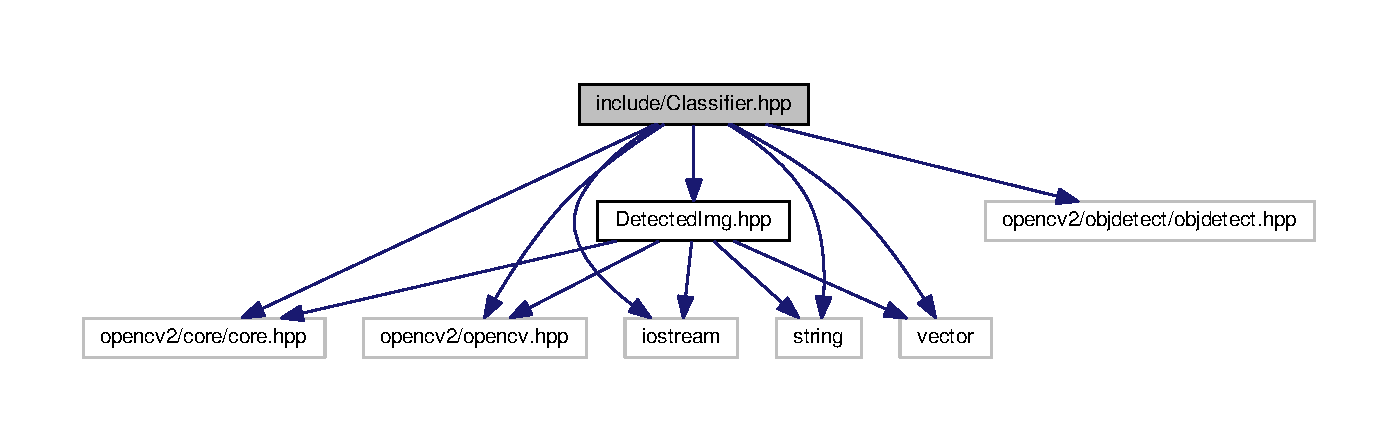
\includegraphics[width=350pt]{Classifier_8hpp__incl}
\end{center}
\end{figure}
This graph shows which files directly or indirectly include this file\+:
\nopagebreak
\begin{figure}[H]
\begin{center}
\leavevmode
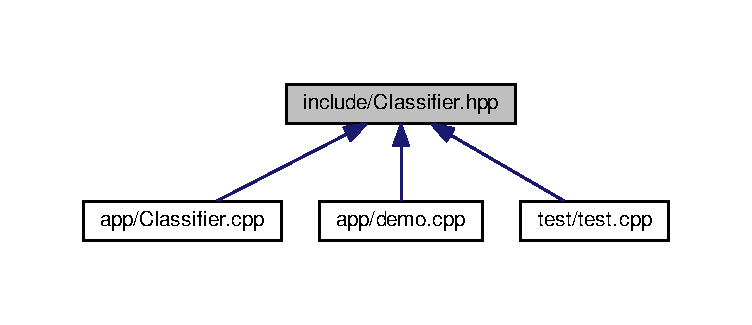
\includegraphics[width=350pt]{Classifier_8hpp__dep__incl}
\end{center}
\end{figure}
\subsection*{Classes}
\begin{DoxyCompactItemize}
\item 
class \hyperlink{classClassifier}{Classifier}
\end{DoxyCompactItemize}

\hypertarget{ContactInfo_8hpp}{}\section{include/\+Contact\+Info.hpp File Reference}
\label{ContactInfo_8hpp}\index{include/\+Contact\+Info.\+hpp@{include/\+Contact\+Info.\+hpp}}
{\ttfamily \#include $<$iostream$>$}\\*
{\ttfamily \#include $<$vector$>$}\\*
{\ttfamily \#include $<$string$>$}\\*
Include dependency graph for Contact\+Info.\+hpp\+:\nopagebreak
\begin{figure}[H]
\begin{center}
\leavevmode
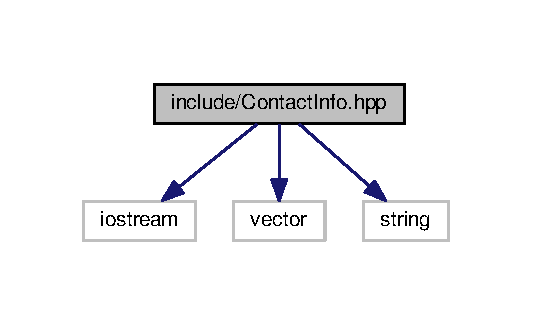
\includegraphics[width=256pt]{ContactInfo_8hpp__incl}
\end{center}
\end{figure}
\subsection*{Classes}
\begin{DoxyCompactItemize}
\item 
class \hyperlink{classContactInfo}{Contact\+Info}
\end{DoxyCompactItemize}

\hypertarget{DetectedImg_8hpp}{}\section{include/\+Detected\+Img.hpp File Reference}
\label{DetectedImg_8hpp}\index{include/\+Detected\+Img.\+hpp@{include/\+Detected\+Img.\+hpp}}


This class is the data container that stores the detected images and its results from S\+VM testing.  


{\ttfamily \#include $<$opencv2/core/core.\+hpp$>$}\\*
{\ttfamily \#include $<$opencv2/opencv.\+hpp$>$}\\*
{\ttfamily \#include $<$iostream$>$}\\*
{\ttfamily \#include $<$string$>$}\\*
{\ttfamily \#include $<$vector$>$}\\*
Include dependency graph for Detected\+Img.\+hpp\+:\nopagebreak
\begin{figure}[H]
\begin{center}
\leavevmode
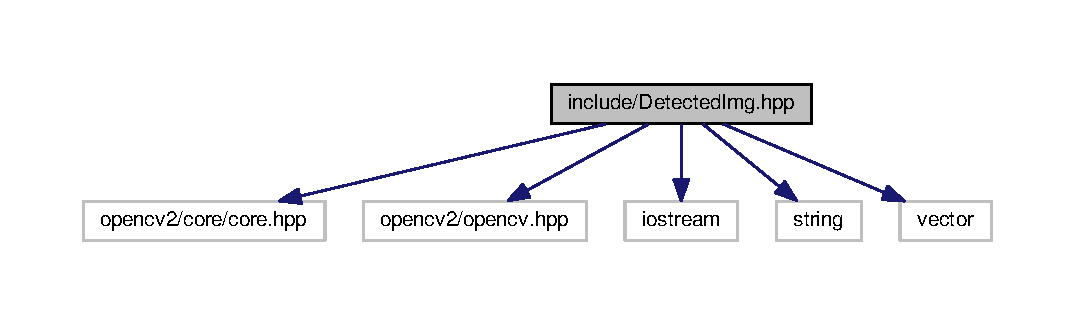
\includegraphics[width=350pt]{DetectedImg_8hpp__incl}
\end{center}
\end{figure}
This graph shows which files directly or indirectly include this file\+:
\nopagebreak
\begin{figure}[H]
\begin{center}
\leavevmode
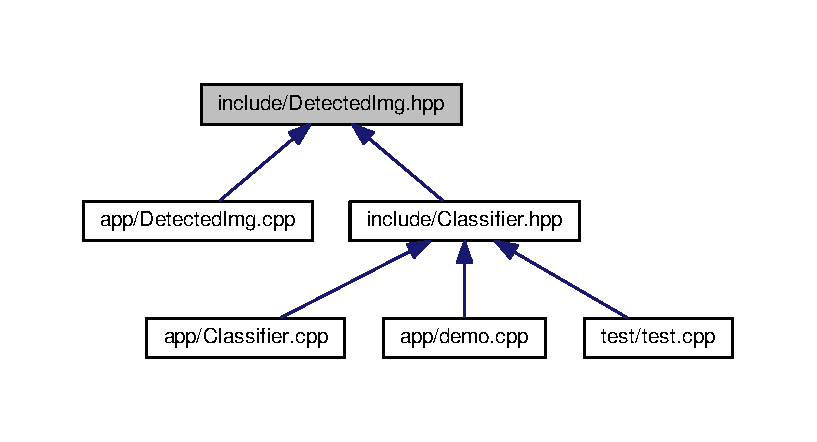
\includegraphics[width=350pt]{DetectedImg_8hpp__dep__incl}
\end{center}
\end{figure}
\subsection*{Classes}
\begin{DoxyCompactItemize}
\item 
class \hyperlink{classDetectedImg}{Detected\+Img}
\end{DoxyCompactItemize}


\subsection{Detailed Description}
This class is the data container that stores the detected images and its results from S\+VM testing. 

\begin{DoxyCopyright}{Copyright}
Copyright 2017 Yuyu Hsueh. All rights reserved. 
\end{DoxyCopyright}

\hypertarget{main_8cpp}{}\section{test/main.cpp File Reference}
\label{main_8cpp}\index{test/main.\+cpp@{test/main.\+cpp}}
{\ttfamily \#include $<$gtest/gtest.\+h$>$}\\*
Include dependency graph for main.\+cpp\+:\nopagebreak
\begin{figure}[H]
\begin{center}
\leavevmode
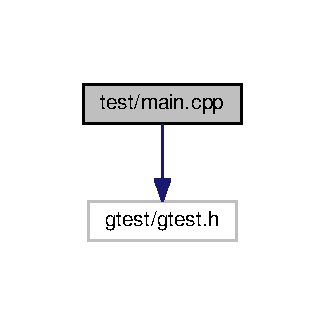
\includegraphics[width=156pt]{main_8cpp__incl}
\end{center}
\end{figure}
\subsection*{Functions}
\begin{DoxyCompactItemize}
\item 
int \hyperlink{main_8cpp_a3c04138a5bfe5d72780bb7e82a18e627}{main} (int argc, char $\ast$$\ast$argv)
\end{DoxyCompactItemize}


\subsection{Function Documentation}
\index{main.\+cpp@{main.\+cpp}!main@{main}}
\index{main@{main}!main.\+cpp@{main.\+cpp}}
\subsubsection[{\texorpdfstring{main(int argc, char $\ast$$\ast$argv)}{main(int argc, char **argv)}}]{\setlength{\rightskip}{0pt plus 5cm}int main (
\begin{DoxyParamCaption}
\item[{int}]{argc, }
\item[{char $\ast$$\ast$}]{argv}
\end{DoxyParamCaption}
)}\hypertarget{main_8cpp_a3c04138a5bfe5d72780bb7e82a18e627}{}\label{main_8cpp_a3c04138a5bfe5d72780bb7e82a18e627}

\hypertarget{test_8cpp}{}\section{test/test.cpp File Reference}
\label{test_8cpp}\index{test/test.\+cpp@{test/test.\+cpp}}


testcpp is used for unit testing  


{\ttfamily \#include \char`\"{}Classifier.\+hpp\char`\"{}}\\*
{\ttfamily \#include $<$opencv2/core/core.\+hpp$>$}\\*
{\ttfamily \#include $<$opencv2/opencv.\+hpp$>$}\\*
{\ttfamily \#include $<$opencv2/objdetect/objdetect.\+hpp$>$}\\*
{\ttfamily \#include $<$gtest/gtest.\+h$>$}\\*
{\ttfamily \#include $<$iostream$>$}\\*
{\ttfamily \#include $<$string$>$}\\*
{\ttfamily \#include $<$vector$>$}\\*
Include dependency graph for test.\+cpp\+:
\nopagebreak
\begin{figure}[H]
\begin{center}
\leavevmode
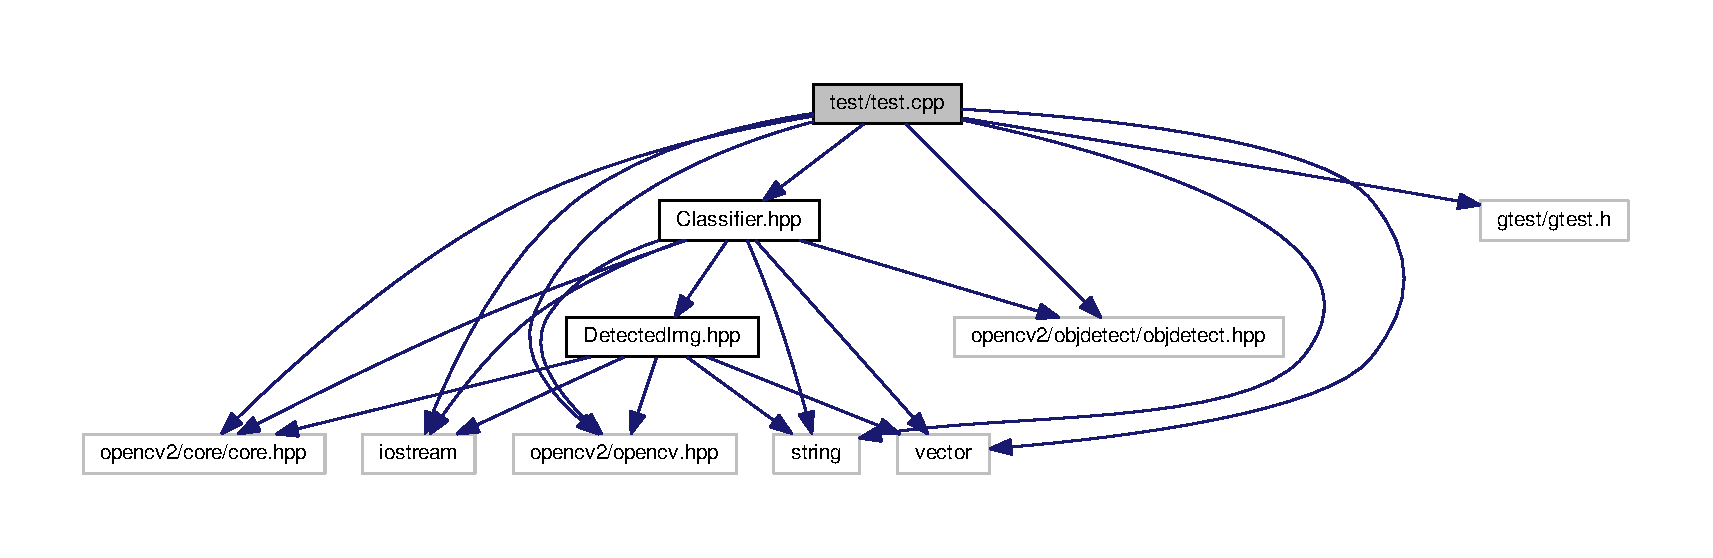
\includegraphics[width=350pt]{test_8cpp__incl}
\end{center}
\end{figure}
\subsection*{Classes}
\begin{DoxyCompactItemize}
\item 
struct \hyperlink{structClassifierTest}{Classifier\+Test}
\item 
struct \hyperlink{structDetectedTest}{Detected\+Test}
\end{DoxyCompactItemize}
\subsection*{Functions}
\begin{DoxyCompactItemize}
\item 
\hyperlink{test_8cpp_a5eb658e8223b643bc351f9ef17a81b4d}{T\+E\+S\+T\+\_\+F} (\hyperlink{structClassifierTest}{Classifier\+Test}, Saved\+Path)
\item 
\hyperlink{test_8cpp_af32d40a8a5e339bd509e68a1a36e303b}{T\+E\+S\+T\+\_\+F} (\hyperlink{structDetectedTest}{Detected\+Test}, load\+Img)
\item 
\hyperlink{test_8cpp_a68654f27a46f08d647d78ec6bdcdf4b6}{T\+E\+S\+T\+\_\+F} (\hyperlink{structDetectedTest}{Detected\+Test}, View\+Set\+Result)
\end{DoxyCompactItemize}


\subsection{Detailed Description}
testcpp is used for unit testing 

\begin{DoxyCopyright}{Copyright}
Copyright 2017 Yuyu Hsueh. All rights reserved. 
\end{DoxyCopyright}


\subsection{Function Documentation}
\index{test.\+cpp@{test.\+cpp}!T\+E\+S\+T\+\_\+F@{T\+E\+S\+T\+\_\+F}}
\index{T\+E\+S\+T\+\_\+F@{T\+E\+S\+T\+\_\+F}!test.\+cpp@{test.\+cpp}}
\subsubsection[{\texorpdfstring{T\+E\+S\+T\+\_\+\+F(\+Classifier\+Test, Saved\+Path)}{TEST_F(ClassifierTest, SavedPath)}}]{\setlength{\rightskip}{0pt plus 5cm}T\+E\+S\+T\+\_\+F (
\begin{DoxyParamCaption}
\item[{{\bf Classifier\+Test}}]{, }
\item[{Saved\+Path}]{}
\end{DoxyParamCaption}
)}\hypertarget{test_8cpp_a5eb658e8223b643bc351f9ef17a81b4d}{}\label{test_8cpp_a5eb658e8223b643bc351f9ef17a81b4d}
\index{test.\+cpp@{test.\+cpp}!T\+E\+S\+T\+\_\+F@{T\+E\+S\+T\+\_\+F}}
\index{T\+E\+S\+T\+\_\+F@{T\+E\+S\+T\+\_\+F}!test.\+cpp@{test.\+cpp}}
\subsubsection[{\texorpdfstring{T\+E\+S\+T\+\_\+\+F(\+Detected\+Test, load\+Img)}{TEST_F(DetectedTest, loadImg)}}]{\setlength{\rightskip}{0pt plus 5cm}T\+E\+S\+T\+\_\+F (
\begin{DoxyParamCaption}
\item[{{\bf Detected\+Test}}]{, }
\item[{load\+Img}]{}
\end{DoxyParamCaption}
)}\hypertarget{test_8cpp_af32d40a8a5e339bd509e68a1a36e303b}{}\label{test_8cpp_af32d40a8a5e339bd509e68a1a36e303b}
\index{test.\+cpp@{test.\+cpp}!T\+E\+S\+T\+\_\+F@{T\+E\+S\+T\+\_\+F}}
\index{T\+E\+S\+T\+\_\+F@{T\+E\+S\+T\+\_\+F}!test.\+cpp@{test.\+cpp}}
\subsubsection[{\texorpdfstring{T\+E\+S\+T\+\_\+\+F(\+Detected\+Test, View\+Set\+Result)}{TEST_F(DetectedTest, ViewSetResult)}}]{\setlength{\rightskip}{0pt plus 5cm}T\+E\+S\+T\+\_\+F (
\begin{DoxyParamCaption}
\item[{{\bf Detected\+Test}}]{, }
\item[{View\+Set\+Result}]{}
\end{DoxyParamCaption}
)}\hypertarget{test_8cpp_a68654f27a46f08d647d78ec6bdcdf4b6}{}\label{test_8cpp_a68654f27a46f08d647d78ec6bdcdf4b6}

%--- End generated contents ---

% Index
\backmatter
\newpage
\phantomsection
\clearemptydoublepage
\addcontentsline{toc}{chapter}{Index}
\printindex

\end{document}
